\documentclass[11pt,letterpaper]{article}
\usepackage[T1]{fontenc}\usepackage[utf8]{inputenc}\usepackage{lmodern,microtype}
\usepackage[margin=1in]{geometry}\usepackage{graphicx,booktabs,array,amsmath,amssymb,amsthm,caption,longtable,pdflscape}
\usepackage[numbers,sort&compress]{natbib}
\usepackage[hidelinks]{hyperref}
\captionsetup{font=small,labelfont=bf,justification=raggedright,singlelinecheck=false}
\newcommand{\SpO}{SpO\textsubscript{2}}\newcommand{\tightnote}[1]{\par\smallskip{\footnotesize\raggedright #1\par}}
\renewcommand{\thetable}{S\arabic{table}}\renewcommand{\thefigure}{S\arabic{figure}}
\renewcommand{\arraystretch}{1.1}\setlength{\tabcolsep}{4pt}\setlength{\emergencystretch}{2em}
\graphicspath{{../}{./}}\newcommand{\figalt}[1]{\par\smallskip{\footnotesize\textit{Alt text:} #1\par}}

% ---- inlined from 02_supp/_blocks/figures_supp.tex ----
\newcommand{\FigFlow}{\begin{figure}[!htbp]\centering
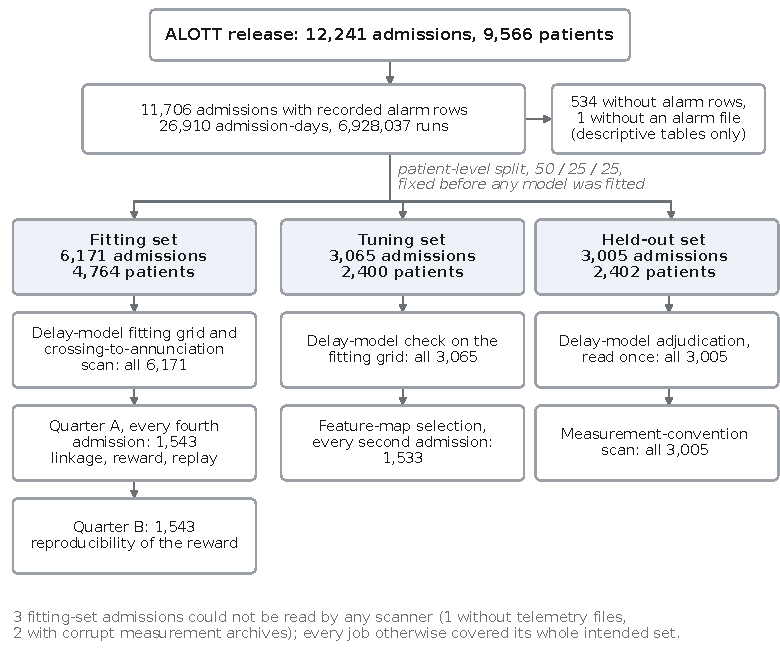
\includegraphics[width=\textwidth]{figures/FigureS1_study_flow.pdf}
\caption{Study flow from the release to the analysis sets. Counts are the intended cohort of each scan job as recorded in the analysis records; admissions rather than patients define the every-fourth-admission quarters of the fitting set and the every-second-admission subsample of the tuning set. The delay model was fitted on the fitting grid, checked on the tuning set and evaluated once on the held-out set; linked-reward calibration used quarter A of the fitting set with the feature map selected on the tuning subsample.}
\label{sfig:flow}
\figalt{A flow diagram. The release of 12,241 admissions and 9,566 patients splits into fitting, tuning and held-out sets of 6,171, 3,065 and 3,005 admissions. Under the fitting set sit the delay-model grid and crossing scan on all admissions, quarter A of 1,543 admissions for linkage, reward and replay, and quarter B of 1,543 for reproducibility; under the tuning set the delay-model check and the feature-map subsample of 1,533; under the held-out set the single assessment and the convention scan. A note records three fitting-set admissions no scanner could read.}
\end{figure}}
\newcommand{\FigFitGrid}{\begin{figure}[!htbp]\centering
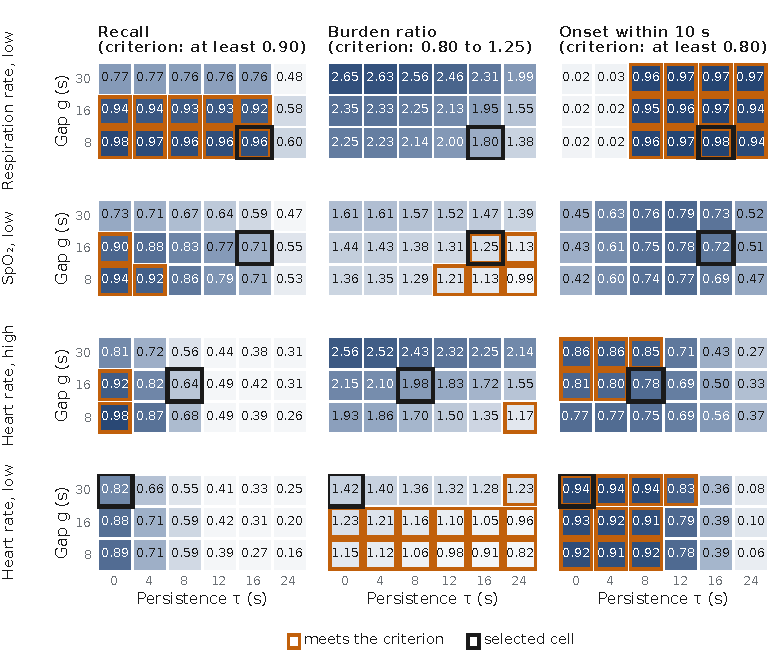
\includegraphics[width=\textwidth]{figures/FigureS2_fit_grid.pdf}
\caption{The delay-model fitting grid against the three validation criteria. One row per channel, one panel per criterion; each cell is a persistence--gap pair $(\tau,g)$ of the grid, shaded and labelled by its pooled fitting-set value. Cells that meet the criterion are outlined, and the cell the tuning-checked $F_1$ selection kept carries a heavy border. The criteria were fixed before the held-out data were examined; the held-out assessment is shown in main Figure 3 of the main manuscript.}
\label{sfig:fitgrid}
\figalt{Twelve small grids of six by three cells. Recall is high only at short persistence and falls with it; burden ratios lie above the 0.80 to 1.25 band at every cell on respiration rate low and at all but one cell on heart rate high, and enter it at long persistence or short gaps on the other channels; onset agreement is high at long persistence on respiration rate and at short persistence on the heart-rate channels. No cell is outlined in all three panels of any row.}
\end{figure}}
\newcommand{\FigConventions}{\begin{figure}[!htbp]\centering
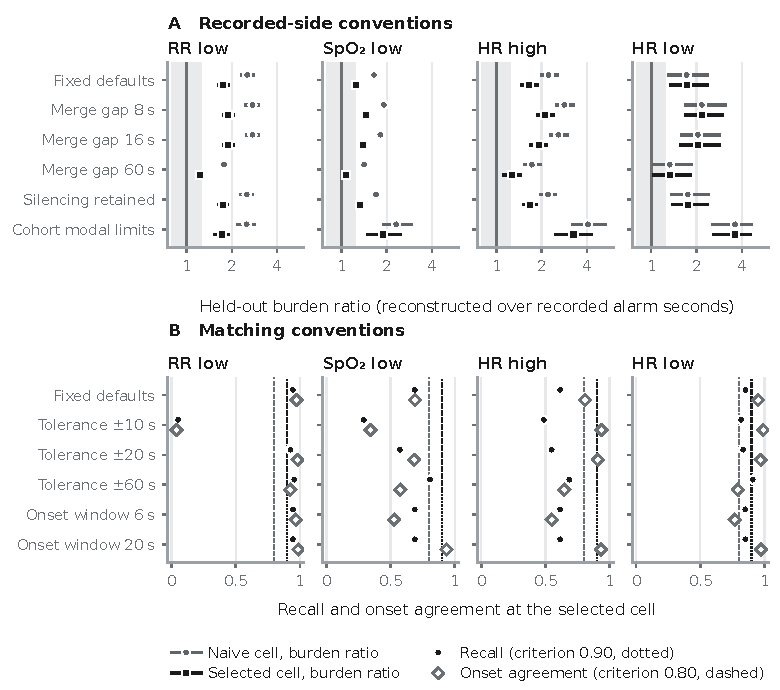
\includegraphics[width=\textwidth]{figures/FigureS3_conventions.pdf}
\caption{The measurement-convention scan, one convention varied at a time from the fixed defaults. A: held-out burden ratio for the naive and the selected cell under the recorded-side conventions, with 95\% patient-cluster bootstrap intervals; the shaded band is the prespecified validation range. B: episode recall and onset agreement at the selected cell under the matching conventions, which leave the burden ratio unchanged by construction; the dotted and dashed lines are the two criteria. Tables~\ref{stab:convA} and~\ref{stab:convB} give the values.}
\label{sfig:conventions}
\figalt{Eight panels of dot plots, one per channel in each of two rows. In the upper row the burden ratios lie above the validation band except at the 60-second merge gap, where the selected cell enters it on respiration rate low and oxygen saturation low; cohort modal limits raise the ratios most. In the lower row recall and onset agreement move with the matching tolerance and onset window, and the tight 10-second tolerance collapses both on respiration rate low.}
\end{figure}}
\newcommand{\FigLag}{\begin{figure}[!htbp]\centering
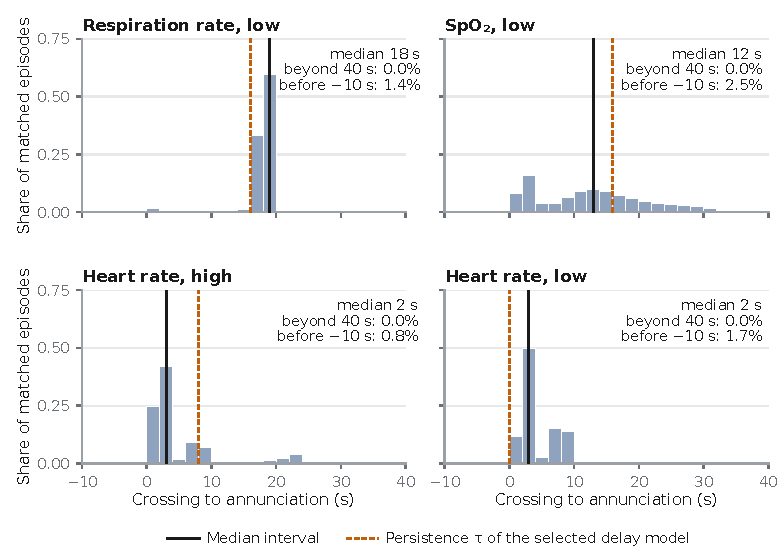
\includegraphics[width=\textwidth]{figures/FigureS4_lag.pdf}
\caption{Time from the numeric crossing to the recorded annunciation, by channel: the share of matched episodes in each two-second bin on the whole fitting set at the naive setting, with the median and, for reference, the persistence $\tau$ of the selected delay model. Positive values mean the monitor annunciated after the crossing; the shares outside the window shown are annotated. Table~\ref{stab:crossing} gives the quantiles.}
\label{sfig:lag}
\figalt{Four histograms. Respiration rate low is concentrated at 16 to 18 seconds; heart rate high and heart rate low peak at 0 to 4 seconds with short right tails; oxygen saturation low is spread from 0 to about 30 seconds with a mode near 2 seconds and a broad hump around 12 seconds. Almost no episodes fall before minus 10 seconds or beyond 40 seconds.}
\end{figure}}
\newcommand{\FigGrid}{\begin{figure}[!htbp]\centering
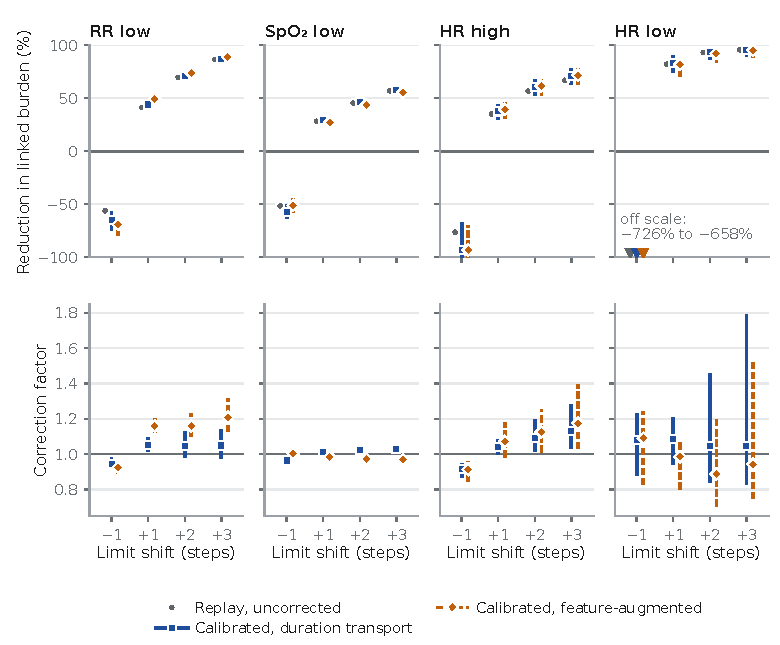
\includegraphics[width=\textwidth]{figures/FigureS5_grid.pdf}
\caption{Replay and linked-reward calibration over the full limit-shift grid. Upper row: replayed and calibrated reductions in linked burden, with 95\% patient-cluster intervals for the two cell-standardised estimates; the more stringent heart-rate-low comparison lies off the scale and is annotated. Lower row: the correction factors $\hat\kappa$ and $\hat\kappa_z$ with their intervals, against one. Main-manuscript Figure 5 is the one-step column of the upper row; Table~\ref{tab:tworoutesfull} gives the values, the coarsened shares and the fixed-offset comparator.}
\label{sfig:grid}
\figalt{Two rows of four panels. At one step the reductions range from about 27 percent on oxygen saturation low to 84 percent on heart rate low, and at three steps from 55 to 96 percent, with calibrated estimates close to replay; the one-step-more-stringent shift gives negative reductions. Correction factors lie between about 0.9 and 1.2 with intervals that widen with the shift, widest on heart rate low, and the feature-augmented factor exceeds the duration-transport factor on respiration rate low.}
\end{figure}}

% ---- end inline ----

\title{\bfseries Supplementary Methods and Results\\[5pt]\large
% ---- inlined from 02_supp/../shared/title.tex ----
Alarm burden beyond threshold replay: linked-reward calibration of recorded clinical alarms

% ---- end inline ----
}
\author{Zihao Wang \and Michele Ceccarelli \and Min Lu}\date{}
\begin{document}\maketitle
\noindent This supplement documents cohort accounting, reconstruction conventions, additional validation, and the diagnostics underlying the cell-calibrated comparisons. Implementation details accompany the diagnostics in the relevant sections below. The simulation is reproducible from the supplied code; independent re-creation of the clinical analyses requires credentialed ALOTT access and the fixed analysis records.
\setcounter{tocdepth}{1}\tableofcontents

\section{Cohort and recorded burden}\label{s:cohort}

% ---- inlined from 02_supp/_blocks/P1_cohort_burden.tex ----
\subsection{Cohort accounting}
Of 12\,241 admissions, 11\,706 contributed at least one alarm row and
span 26\,910 admission-days; 534 had an alarm file without alarm rows and one had no alarm file
(Table~\ref{tab:cohort}), contributing neither burden nor denominator in the descriptive burden tables. The patient-level split was applied to all 12\,241 admissions, independently of this descriptive restriction. Descriptive analyses stratify by an
admission-level \emph{oncology tier} defined from the release's
discharge diagnosis codes --- \emph{strict oncology}, a malignant ICD-10-CM code in the primary or
secondary field (1\,919 admissions, 1\,679 patients); \emph{oncology context}, a cancer-related code or
diagnosis term without a malignant code (1\,389 admissions); and \emph{non-oncology} --- and, within the
strict cohort, by the cancer group of the first malignant code (haematological 248, thoracic 276,
gastrointestinal 525, other solid 870 admissions; code ranges in Section~\ref{s:oncology}). Codes are discharge
coding, used for cohorting only.


\subsection{Recorded alarm burden and silencing}

Across 11\,706 alarm-bearing admissions and 26\,910 admission-days, monitors
recorded 257 alarm runs per admission-day: numeric-limit 93.9, arrhythmia
82.2, technical 45.6 and system 35.8 (Table~\ref{tab:burden}). Technical states
comprise about 18\% of events and half of alarm-active time
, because states such as lead failure and pulse
search persist for hours once entered.

The most frequent single alarm type is respiration rate high, at 28.3 runs per
admission-day  --- the channel excluded from all replay
analyses. Recorded silencing occupies 4.5\% of alarm-active time overall,
varies by class (2.0\% arrhythmia to 6.6\% technical) and rises across the
oncology tiers from 4.1\% to 8.1\% (Table~\ref{stab:oncburden}); \SpO{} low is silenced for 15.6\% of its alarm-active
time and heart rate high for 14.9\%.


\subsection{The oncology cohort}

Recorded burden per admission-day was similar across tiers (236, 269 and 257
runs in strict-oncology, oncology-context and non-oncology admissions;
Tables~\ref{stab:oncburden} and~\ref{stab:oncchannel}), but strict-oncology admissions carried fewer
numeric-limit runs (81.7 versus 93.4 per admission-day), more \SpO{}-low,
respiration-rate-low and technical runs, and about twice the silenced share on
every numeric-limit channel (\SpO{} low 34.7\% against 13.9\% of alarm-active
time; heart rate high 26.5\% against 13.5\%). Within the strict cohort,
thoracic admissions generate the most \SpO{}-low runs (16.5 per admission-day
against 8.0--9.5 elsewhere), and haematological admissions the most
heart-rate-high runs (7.4) and the highest silenced share (12.5\%).


\begin{table}[htbp]\centering\small
\caption{Cohort, recorded alarm data, and the patient-disjoint split.}
\label{tab:cohort}
\begin{tabular}{lrrr}
\toprule
 & Patients & Admissions & Admission-days \\
\midrule
Study telemetry cohort & 9\,566 & 12\,241 & --- \\
\quad With recorded alarm rows & --- & 11\,706 & 26\,910 \\
\quad Alarm file present, no alarm rows & --- & 534 & --- \\
\quad No alarm file & --- & 1 & --- \\
\addlinespace
Fitting set & 4\,764 & 6\,171 & --- \\
Tuning set & 2\,400 & 3\,065 & --- \\
Test set & 2\,402 & 3\,005 & --- \\
\bottomrule
\end{tabular}
\tightnote{The split is at the patient level, allocated 50/25/25 by a
deterministic pseudorandom rule, and was fixed together with the candidate
parameter grid and every adequacy criterion before any model was fitted. Admission-days are spanned by recorded alarm rows (floor one
hour), on the calendar. Admissions with no alarm rows contribute neither burden nor denominator
and are reported, not imputed.}
\end{table}


\begin{table}[htbp]\centering\small
\caption{Recorded alarm burden and silencing, by alarm class.}
\label{tab:burden}
\begin{tabular}{lrrrrrr}
\toprule
Alarm class & Annunciation & Runs per & Alarm-min per & Share of & Share of & Silenced share \\
 & runs & adm-day & adm-day & runs & alarm time & of alarm time \\
\midrule
Numeric limit & 2\,527\,205 & 93.9 & 189 & 36\% & 28\% & 3.2\% \\
Arrhythmia & 2\,210\,599 & 82.2 & 98 & 32\% & 15\% & 2.0\% \\
Technical & 1\,228\,233 & 45.6 & 338 & 18\% & 50\% & 6.6\% \\
System & 962\,000 & 35.8 & 51 & 14\% & 8\% & 0.0\% \\
\midrule
All classes & 6\,928\,037 & 257.5 & 677 & 100\% & 100\% & 4.5\% \\
\bottomrule
\end{tabular}
\tightnote{11\,706 admissions, 26\,910 admission-days. An annunciation run is a
maximal sequence of alarm-active rows separated by no more than 30\,s. Silenced
share is silenced alarm-active seconds divided by total alarm-active seconds.}
\end{table}










% ---- end inline ----


\section{Data allocation and reproducibility}\label{s:split}\label{s:seeds}

% ---- inlined from 02_supp/_blocks/P1_seeds.tex ----
Patient splitting and systematic admission subsampling are deterministic given the analysis record. The split has 4\,764 fitting, 2\,400 tuning and 2\,402 held-out patients. The primary calibration subsample comprises every fourth fitting-set admission in the fixed processing order; a different admission quarter is used for reproducibility. Admissions rather than patients define these quarters, so the quarters are not asserted to be patient-disjoint.

The held-out percentile intervals use 400 patient bootstrap samples with seed 20260831. Stability analyses use 2\,000 samples under seeds 20260831, 7 and 12345. All admissions remain attached to their patient during resampling. The descriptive crossing-to-annunciation scan uses the whole fitting set (6\,171 admissions, 239\,061 matched episodes). Calibration and simulation seeds and settings are specified in the analysis code. Exact numerical reproduction additionally requires the credentialed source data, the fixed split record and the documented software environment.

% ---- end inline ----

Figure~\ref{sfig:flow} shows the allocation from the release to the analysis sets, with the intended cohort of every scan job.
\FigFlow
The delay-model class, parameter grid and validation criteria were fixed before analysis of held-out data. Development used fitting patients, with a tuning-set check before the held-out assessment. Linked-reward calibration was developed subsequently using fitting data, with an independent tuning map for feature estimation. These distinct stages should not be described as one prospectively registered calibration analysis.

\section{Run construction and linkage}\label{s:defs}

% ---- inlined from 02_supp/_blocks/S1_persistence_monotone.tex ----
Fix an admission and a merge gap $g$. Let $\mathcal C_g$ be the set of crossing runs after merging. A persistence rule retains runs with duration at least $\tau$; it does not change their endpoints. Recorded and reconstructed active seconds are sums of run durations under their respective stated conventions.

\textbf{Monotonicity property S1.} For $\tau\le\tau'$, the retained run set under $\tau'$ is a subset of the set under $\tau$. Run count and active seconds cannot increase. The number of recorded episodes overlapped by at least one retained run, and hence recorded-episode recall, cannot increase. Precision has no general monotonicity.

\emph{Proof.} The sets $\{r\in\mathcal C_g:|r|\ge\tau\}$ are nested. Deleting runs cannot create an overlap for a previously unmatched recorded episode. Precision can increase when a short unmatched run is deleted or decrease when a short matched run is deleted while longer unmatched runs remain. Both constructions can leave a positive denominator. $\square$

% ---- end inline ----


% ---- inlined from 02_supp/_blocks/S2_mergegap_monotone.tex ----
\textbf{Monotonicity property S2.} With no persistence filter, increasing the merge gap cannot increase run count and cannot decrease active seconds. If two runs whose final and initial active timestamps are separated by $\gamma$ seconds are merged, the added duration is $\gamma-\Delta\ge0$, where $\Delta$ is the nominal sampling interval and the gaps considered are at least $\Delta$.

\emph{Proof.} The separate durations sum to $(e_1-s_1+\Delta)+(e_2-s_2+\Delta)$; the merged duration is $e_2-s_1+\Delta$. Their difference is $s_2-e_1-\Delta$. Repeating the calculation proves the claim. $\square$

When only the recorded-side gap is increased, the reconstructed-to-recorded active-second ratio cannot increase. This statement concerns a measurement convention, not an improvement in physiological event detection.

% ---- end inline ----

\subsection{Zero-inclusive linkage}\label{s:linkdef}
% ---- inlined from 02_supp/_blocks/P1_linkage_rule.tex ----
For linked-reward calibration, retain timestamps at which the value crosses the contemporaneous limit. Successive crossing timestamps separated by at most 4 seconds belong to the same excursion, even if a brief intervening sample is not a crossing. Excursion duration is the last minus first crossing timestamp plus the nominal two-second sample interval. Recorded silenced and inactive periods are excluded before constructing both streams. Recorded alarm runs are formed by the same four-second gap convention.

For a recorded run with onset $A_s$ and final active timestamp $A_e$, eligible excursions must start in $[A_s-30,A_e]$. The run is assigned to the excursion in this set with the largest positive endpoint overlap, $\min(A_e,e)-\max(A_s,s)>0$, with processing order resolving ties. Duration accounting subsequently adds the nominal two-second interval. The onset-search restriction is part of the estimand-defining convention; the analysis does not search every earlier excursion that might overlap a long alarm. A run may be assigned at most once; an excursion may receive several runs. The excursion reward is the sum of assigned run durations, not the envelope from the first alarm onset to the last alarm end. Unassigned run seconds are retained separately. The onset lag uses the earliest assigned onset, and extension uses the latest assigned termination. The implementation is \texttt{scan/scan\_linkage.py}. Its output includes every replayed excursion, including those with zero linked reward.

\paragraph{Time and overshoot.} Timestamps are read as elapsed calendar time on the coordinate the release records; an explicit offset is normalised and none is inferred, so a run in progress at midnight at the end of a month is one run. The overshoot of an excursion is the maximal directed excess of its eligible crossing samples beyond the limit in force at each sample, left unrounded until it is binned; silenced or inactivated samples that the four-second gap bridges do not enter it, and neither do samples that do not cross. These are the conventions the counterfactual replay used throughout. An earlier implementation of the timestamp parser and of the excursion-feature routine departed from them --- the parser treated every month as 31 days long, so a run in progress at the end of a shorter month was cut in two, and the feature routine measured the excess against the limit in force at the excursion's start over every sample of the excursion's window --- and every analysis in this paper was recomputed after the correction, under the design fixed in advance and with the same splits, selected model, cell-map rule and seeds. The correction touched the recorded alarm runs of 58 admissions, the replayed excursions of one fitting-set admission, the delay-model matching of three fitting-set and one held-out admission, the overshoot bin of fewer than twenty admission--channel pairs in each analysis subsample, and the monitored spans of the 268 admissions whose stay crossed the end of a month shorter than 31 days; the largest movement in a reported calibrated reduction is 0.3 percentage points, the per-admission-day rates of Section~\ref{s:cohort} rose by about one per cent, and no conclusion changed.

% ---- end inline ----

\subsection{Validation algorithm}\label{s:algorithm}
% ---- inlined from 02_supp/_blocks/S6_reconstruction_algorithm.tex ----
The validation algorithm and the linked-reward algorithm serve different purposes. Validation allows a persistence requirement and evaluates onset agreement; linked-reward calibration retains all eligible excursions, including short and unannunciated ones.
\begin{enumerate}\itemsep2pt
\item Carry forward the most recently recorded applicable alarm limit. Exclude implausible values and recorded silenced or inactive periods.
\item Group crossing timestamps using the candidate gap $g$ and retain runs with duration at least $\tau$. Group recorded alarm-active rows using the fixed 30-second validation gap.
\item Match recorded episodes to overlapping reconstructed episodes within the stated tolerance. Score onset agreement using the reconstructed onset shifted by $\tau$, within 10 seconds of the recorded onset.
\item Aggregate counts, active seconds and onset agreement within patient, keeping all admissions of that patient together. Use ratios of pooled patient totals, rather than unweighted means of admission-specific ratios.
\end{enumerate}
For the subsequent calibration, use the four-second linkage rule in Section~\ref{s:linkdef}, without a persistence filter. Matching for validation must not be substituted for this zero-inclusive reward construction.

% ---- end inline ----

\subsection{Ratio inference}\label{s:ratio}
% ---- inlined from 02_supp/_blocks/S3_ratio_inference.tex ----
\textbf{Inference note S3.} \emph{Let $(X_i,Y_i)$ be i.i.d.\ patient-cluster aggregates with
$\mu_Y=\mathbb E[Y_i]>0$ and finite second moments, and $\hat\rho=\sum X_i/\sum Y_i$,
$\rho=\mu_X/\mu_Y$. Then $\sqrt n(\hat\rho-\rho)\rightarrow N(0,\sigma^2)$ with
$\sigma^2=\mu_Y^{-2}\,\mathrm{Var}(X_i-\rho Y_i)$, and the nonparametric cluster bootstrap consistently
estimates this law.}

\emph{Proof.} Delta method applied to $(\bar X,\bar Y)\mapsto\bar X/\bar Y$ at $(\mu_X,\mu_Y)$; bootstrap
consistency for smooth functions of means under i.i.d.\ cluster resampling is classical; see
\citet{field2007bootstrapping} for the clustered setting. $\square$

Episode recall, precision, onset agreement and the naive and delay-aware burden ratios are all of this form;
the reported 95\% intervals are percentile intervals over $B=400$ patient resamples; Section~\ref{s:bootstab} repeats
them at $B=2000$ under three seeds.

% ---- end inline ----


\section{Additional held-out validation}\label{s:validation}
The three prespecified criteria were recall at least 0.90, a reconstructed-to-recorded burden ratio in $[0.80,1.25]$, and onset agreement within 10 seconds for at least 0.80 of matched episodes. The delay model would be carried forward only if at least two channels met all three criteria. No channel did so (main Figure 3 of the main manuscript). The additional analyses below characterise the discrepancy without selecting another model on the held-out sample.
\subsection{Bootstrap and influence stability}\label{s:bootstab}

% ---- inlined from 02_supp/_blocks/P2_tab_seedstab.tex ----
\subsection{Monte Carlo and influence stability}
Table~\ref{stab:seedstab} compares the reported $B=400$ intervals with the
$B=2000$ re-run and reports, across the three seeds, the largest movement of either endpoint, together with
the largest relative change in the pooled ratio when any single patient is removed.

\begin{table}[htbp]\centering\footnotesize
\setlength{\tabcolsep}{4pt}
\caption{Bootstrap seed stability and leave-one-patient-out influence of the test-set burden ratios.}
\label{stab:seedstab}
\begin{tabular}{llrllrr}
\toprule
Channel & Cell $(\tau,g)$ & $\hat\rho$ & \multicolumn{2}{c}{95\% CI} & Endpoint drift & LOPO \\
\cmidrule(lr){4-5}
 & & & reported, $B{=}400$ & $B{=}2000$ & (3 seeds) & max $|\Delta\hat\rho|/\hat\rho$ \\
\midrule
RR low   & (0, 30) naive     & 2.53 & 2.27--2.82 & 2.27--2.83 & 0.008 & 3.7\% \\
RR low   & (16, 8) selected  & 1.75 & 1.62--1.92 & 1.61--1.92 & 0.009 & 2.9\% \\
HR high  & (0, 30) naive     & 2.23 & 1.94--2.58 & 1.94--2.59 & 0.033 & 3.7\% \\
HR high  & (8, 16) selected  & 1.65 & 1.46--1.89 & 1.45--1.91 & 0.022 & 3.3\% \\
HR low   & (0, 30) naive $=$ selected & 1.72 & 1.32--2.41 & 1.32--2.47 & 0.066 & 15.4\% \\
\SpO{} low & (0, 30) naive   & 1.65 & 1.57--1.74 & 1.57--1.75 & 0.006 & 1.4\% \\
\SpO{} low & (16, 16) selected & 1.26 & 1.19--1.34 & 1.20--1.34 & 0.007 & 1.9\% \\
\bottomrule
\end{tabular}
\tightnote{RR, respiration rate; HR, heart rate. The $B{=}2000$ interval shown is for seed 20260831;
``endpoint drift'' is the largest movement of either endpoint across seeds 20260831, 7 and 12345; LOPO is
the largest relative change in the pooled ratio when any single patient is removed. Patients contributing
to the test-set ratios: 1\,063 (RR low), 926 (HR high), 1\,410 (\SpO{} low); HR low has the fewest
contributing admissions (700) and is the only channel materially sensitive to one patient. The reported
intervals are those of Figure 3 of the main manuscript of the main text; the re-run is a stability check.}
\end{table}

% ---- end inline ----

\subsection{Admission-level heterogeneity}\label{s:heterog}
% ---- inlined from 02_supp/_blocks/P2_tab_heterog.tex ----
Table~\ref{stab:heterog} summarizes the per-admission naive ratio (reconstructed
divided by recorded alarm-seconds, admissions with nonzero recorded seconds) and the pooled naive ratio
within tertiles of per-admission channel-numerics coverage. Pooled ratios lie below the per-admission
medians because pooling weights admissions by recorded alarm-seconds, and admissions with more recorded
alarm time over-count less.

\begin{table}[htbp]\centering\footnotesize
\setlength{\tabcolsep}{4pt}
\caption{Per-admission heterogeneity of the naive over-count and pooled naive ratios by coverage tertile
(test set).}
\label{stab:heterog}
\begin{tabular}{lrrrrrrr}
\toprule
 & & \multicolumn{3}{c}{Per-admission naive ratio} & \multicolumn{3}{c}{Pooled naive ratio by coverage tertile} \\
\cmidrule(lr){3-5}\cmidrule(lr){6-8}
Channel & Adm. & Median & IQR & Share $>1$ & T1 & T2 & T3 \\
\midrule
RR low     & 1\,180 & 3.28 & 2.20--5.67 & 0.98 & 2.60 (382) & 2.19 (1\,176) & 2.78 (1\,703) \\
HR high    & 1\,075 & 3.06 & 1.41--9.12 & 0.90 & 1.84 (928) & 2.05 (1\,440) & 2.51 (3\,910) \\
HR low     &   700 & 1.00 & 0.35--1.37 & 0.44 & 1.56 (1\,079) & 1.60 (2\,220) & 1.87 (4\,073) \\
\SpO{} low & 1\,620 & 2.00 & 1.48--3.19 & 0.93 & 1.82 (227) & 1.84 (1\,087) & 1.57 (1\,439) \\
\bottomrule
\end{tabular}
\tightnote{Adm., admissions with nonzero recorded alarm-seconds. Tertile cells give the pooled ratio with
the tertile's median minutes of channel numerics coverage in parentheses; cut-points are channel-specific.
Every tertile-level ratio exceeds 1.5.}
\end{table}

% ---- end inline ----

\subsection{Model-component comparisons}\label{s:ablation}
% ---- inlined from 02_supp/_blocks/P2_tab_ablation.tex ----
Model-component comparisons use the fitting grid rather than held-out model reselection. Table~\ref{stab:ablation} gives, for each channel, the selected
two-parameter cell, the best cell with persistence only ($g$ fixed at its naive value 30) and the best cell
with merging only ($\tau=0$), each chosen by pooled $F_1$.

\begin{table}[htbp]\centering\footnotesize
\setlength{\tabcolsep}{4pt}
\caption{Ablation of the two-parameter model on the fitting grid: selected cell versus best single-parameter
cells.}
\label{stab:ablation}
\begin{tabular}{llrrrrr}
\toprule
Channel & Cell $(\tau,g)$ & $F_1$ & Recall & Precision & Burden ratio & Onset $\le 10$\,s \\
\midrule
Respiration rate, low & (16, 8) selected            & 0.881 & 0.958 & 0.816 & 1.795 & 0.978 \\
                      & (16, 30) persistence only   & 0.746 & 0.756 & 0.735 & 2.307 & 0.972 \\
                      & (0, 16) merging only        & 0.566 & 0.944 & 0.404 & 2.347 & 0.018 \\
\addlinespace
Heart rate, high      & (8, 16) selected            & 0.472 & 0.645 & 0.372 & 1.976 & 0.778 \\
                      & (4, 30) persistence only    & 0.452 & 0.715 & 0.330 & 2.523 & 0.860 \\
                      & (0, 30) merging only (naive)& 0.419 & 0.812 & 0.282 & 2.565 & 0.859 \\
\addlinespace
Heart rate, low       & (0, 30) selected = naive    & 0.681 & 0.816 & 0.585 & 1.420 & 0.942 \\
\addlinespace
\SpO{}, low           & (16, 16) selected           & 0.647 & 0.709 & 0.595 & 1.248 & 0.715 \\
                      & (16, 30) persistence only   & 0.563 & 0.591 & 0.538 & 1.471 & 0.733 \\
                      & (0, 16) merging only        & 0.481 & 0.900 & 0.328 & 1.438 & 0.432 \\
\bottomrule
\end{tabular}
\tightnote{Pooled fitting-set metrics. For heart rate low every single-parameter cell coincides with the
selected (naive) cell. Onset agreement is scored after the $\tau$ shift, which is why merging-only cells
on the persistence-type channels place onsets outside the 10-second window.}
\end{table}

% ---- end inline ----

Figure~\ref{sfig:fitgrid} shows the whole fitting grid against the three criteria: no cell meets all three on any channel, and wherever the burden criterion is met, recall falls below 0.90.
\FigFitGrid
\subsection{Measurement conventions}\label{s:convscan}\FigConventions
% ---- inlined from 02_supp/_blocks/S9_convention_results.tex ----
The prespecified convention scan varied recorded-side merge gaps, matching tolerance, onset windows, silencing handling and limit reconstruction, one component at a time. It did not reselect the delay model. The numerical discrepancies persisted, although their magnitudes depended on the convention (Tables~\ref{stab:convA} and~\ref{stab:convB}). Increasing the recorded-run merge gap reduced the reconstructed-to-recorded burden ratio, as the merge-gap monotonicity property predicts. Retaining silenced samples changed ratios by at most 6\%. Using a single cohort modal limit rather than the available individual history increased the discrepancy on three channels. No tested convention led at least two channels to meet all three original criteria.

\begin{landscape}
\begin{table}[htbp]\centering\scriptsize
\setlength{\tabcolsep}{2.5pt}
\caption{Measurement-convention scan, part A: test-set burden ratios (95\% patient-cluster bootstrap intervals, $B=1000$) under perturbations of the recorded-side merge gap, silencing handling and limit convention.}
\label{stab:convA}
\begin{tabular}{lllllllll}
\toprule
 & \multicolumn{2}{c}{RR low} & \multicolumn{2}{c}{HR high} & \multicolumn{2}{c}{HR low} & \multicolumn{2}{c}{\SpO{} low} \\
\cmidrule(lr){2-3} \cmidrule(lr){4-5} \cmidrule(lr){6-7} \cmidrule(lr){8-9}
Convention & naive & selected & naive & selected & naive & selected & naive & selected \\
\midrule
Fixed defaults & 2.53 (2.27--2.83) & 1.75 (1.61--1.92) & 2.23 (1.96--2.59) & 1.65 (1.44--1.90) & 1.72 (1.29--2.40) & 1.72 (1.32--2.40) & 1.65 (1.57--1.74) & 1.26 (1.20--1.34) \\
$\delta_0=8$\,s & 2.75 (2.44--3.07) & 1.90 (1.75--2.09) & 2.83 (2.49--3.31) & 2.09 (1.84--2.44) & 2.17 (1.66--3.16) & 2.17 (1.66--3.05) & 1.92 (1.82--2.03) & 1.46 (1.39--1.55) \\
$\delta_0=16$\,s & 2.74 (2.46--3.05) & 1.90 (1.74--2.08) & 2.58 (2.27--3.00) & 1.91 (1.67--2.19) & 2.04 (1.56--2.88) & 2.04 (1.55--2.88) & 1.82 (1.73--1.93) & 1.38 (1.32--1.47) \\
$\delta_0=60$\,s & 1.77 (1.68--1.89) & 1.23 (1.18--1.29) & 1.72 (1.51--2.00) & 1.27 (1.10--1.48) & 1.33 (1.02--1.89) & 1.33 (1.01--1.85) & 1.42 (1.35--1.50) & 1.08 (1.02--1.14) \\
Silencing retained & 2.51 (2.25--2.80) & 1.74 (1.60--1.91) & 2.20 (1.95--2.52) & 1.67 (1.49--1.89) & 1.75 (1.35--2.45) & 1.75 (1.37--2.42) & 1.69 (1.62--1.78) & 1.33 (1.26--1.39) \\
Cohort modal limits & 2.51 (2.14--2.88) & 1.72 (1.50--1.94) & 4.07 (3.14--5.39) & 3.26 (2.44--4.36) & 3.61 (2.50--4.72) & 3.61 (2.56--4.67) & 2.32 (1.89--2.98) & 1.90 (1.47--2.53) \\
\bottomrule
\end{tabular}
\tightnote{One perturbation at a time from the fixed defaults ($\delta_0=30$\,s; silenced and inactivated samples excluded from both sides; limits carried forward from recorded changes). Matching tolerance and onset window leave burden ratios unchanged by construction and are reported in part B. For heart rate low the selected cell is the naive cell. Cohort modal limits: heart rate high 135, heart rate low 45, \SpO{} low 87, respiration rate low 8.}
\end{table}
\end{landscape}

\begin{table}[htbp]\centering\scriptsize
\setlength{\tabcolsep}{3pt}
\caption{Measurement-convention scan, part B: episode recall and onset agreement at the selected cell under perturbations of the matching tolerance and the onset window (test set).}
\label{stab:convB}
\begin{tabular}{lrrrrrrrr}
\toprule
 & \multicolumn{2}{c}{RR low} & \multicolumn{2}{c}{HR high} & \multicolumn{2}{c}{HR low} & \multicolumn{2}{c}{\SpO{} low} \\
\cmidrule(lr){2-3} \cmidrule(lr){4-5} \cmidrule(lr){6-7} \cmidrule(lr){8-9}
Convention & recall & onset & recall & onset & recall & onset & recall & onset \\
\midrule
Fixed defaults & 0.947 & 0.975 & 0.615 & 0.808 & 0.852 & 0.951 & 0.689 & 0.691 \\
Tolerance $\pm10$\,s & 0.050 & 0.038 & 0.488 & 0.938 & 0.818 & 0.990 & 0.291 & 0.344 \\
Tolerance $\pm20$\,s & 0.928 & 0.984 & 0.549 & 0.909 & 0.834 & 0.970 & 0.573 & 0.684 \\
Tolerance $\pm60$\,s & 0.958 & 0.927 & 0.687 & 0.648 & 0.907 & 0.792 & 0.807 & 0.576 \\
Onset window 6\,s & 0.947 & 0.969 & 0.615 & 0.549 & 0.852 & 0.767 & 0.689 & 0.528 \\
Onset window 20\,s & 0.947 & 0.989 & 0.615 & 0.935 & 0.852 & 0.972 & 0.689 & 0.937 \\
\bottomrule
\end{tabular}
\tightnote{Fixed defaults: matching tolerance $\pm30$\,s, onset window 10\,s. Recall is the matched fraction of recorded runs; onset agreement is the fraction of matched pairs whose onsets (after the $\tau$ shift) fall within the window.}
\end{table}

% ---- end inline ----

Figure~\ref{sfig:conventions} draws both parts of the scan.

\section{Diagnosis-derived population descriptions}\label{s:oncology}
The oncology strata are descriptive discharge-code groups, not randomly assigned exposure groups. Differences in silencing or burden cannot establish a causal effect of cancer status or alarm handling. They show why a common reward mechanism across patient populations should not be assumed without examination.

% ---- inlined from 02_supp/_blocks/front_oncology_burden_table.tex ----
\begin{table}[htbp]\centering\footnotesize
\setlength{\tabcolsep}{4pt}
\caption{Recorded alarm burden and silencing by oncology tier, and by cancer group within the strict-oncology
cohort (alarm-bearing admissions, full release).}
\label{stab:oncburden}
\setlength{\tabcolsep}{3pt}
\begin{tabular}{lrrrrrrrr}
\toprule
 & & & & \multicolumn{4}{c}{Runs per admission-day by class} & \\
\cmidrule(lr){5-8}
Stratum & Adm. & Adm.-days & Runs/day & Num.\ limit & Rhythm & Tech. & System & Silenced \\
\midrule
Strict oncology & 1\,739 & 1\,326.6 & 235.6 & 81.7 & 61.1 & 57.2 & 35.6 & 8.1\% \\
Oncology context & 1\,291 & 2\,838.4 & 269.0 & 103.9 & 85.1 & 44.8 & 35.1 & 5.7\% \\
Non-oncology & 8\,676 & 22\,745.1 & 257.3 & 93.4 & 83.0 & 45.1 & 35.8 & 4.1\% \\
\addlinespace
\multicolumn{9}{l}{\emph{Strict-oncology cohort by cancer group}} \\
Haematological & 234 & 204.8 & 248.2 & 93.8 & 57.3 & 57.6 & 39.5 & 12.5\% \\
Thoracic & 258 & 207.3 & 276.2 & 93.6 & 80.9 & 62.9 & 38.8 & 8.4\% \\
Gastrointestinal & 483 & 353.0 & 178.0 & 52.3 & 40.4 & 56.1 & 29.2 & 7.2\% \\
Other solid & 764 & 561.6 & 252.3 & 91.5 & 68.1 & 55.7 & 37.1 & 7.4\% \\
\bottomrule
\end{tabular}
\tightnote{Tiers and cancer groups are admission-level classifications from the release's discharge diagnosis
fields (Section~\ref{s:cohort}); the release carries no facility or unit labels. Admission-days are the span of
the admission's alarm stream in the release (minimum one hour), so rates are per day of recorded alarm
stream; strict-oncology admissions have shorter recorded spans (0.76 days per admission against 2.62 for
non-oncology admissions). Alarm-active hours per admission-day: 11.7 (strict), 10.2 (context), 11.4
(non-oncology); 9.5 / 8.9 / 13.7 / 12.3 for the four cancer groups in table order. Silenced share is the fraction of alarm-active time in a recorded silenced or
inactivated state, reported as device state without behavioural interpretation.}
\end{table}

% ---- end inline ----


% ---- inlined from 02_supp/_blocks/S8_oncology.tex ----
The release combines a cancer hospital and a heart hospital without facility labels, so the
oncology strata are admission-level: the strict-oncology tier (malignant ICD-10-CM code C00--C96, C4A, C7A or
C7B in the primary or secondary discharge field), the oncology-context tier (no malignant code but Z51, Z85,
G89.3 or a malignancy term in the diagnosis text) and non-oncology; within the strict tier the first malignant
code defines the cancer group (haematological C81--C96, thoracic C30--C39, gastrointestinal C15--C26, other
solid). Tables~\ref{stab:oncchannel}--\ref{stab:oncgroup} were computed once from the existing
scan rows after adjudication, as descriptive decompositions: no selection, adequacy criterion or
test-set read depends on them.

\begin{table}[htbp]\centering\footnotesize
\setlength{\tabcolsep}{3.5pt}
\caption{Channel-level recorded burden (runs per admission-day) and silenced share of alarm-active time, by
oncology tier and by cancer group within the strict-oncology cohort.}
\label{stab:oncchannel}
\setlength{\tabcolsep}{2.5pt}
\begin{tabular}{lrrrrrrrrrr}
\toprule
 & \multicolumn{5}{c}{Runs per admission-day} & \multicolumn{5}{c}{Silenced share of alarm-active time} \\
\cmidrule(lr){2-6}\cmidrule(lr){7-11}
Stratum & RR low & HR high & HR low & \SpO{} low & RR high & RR low & HR high & HR low & \SpO{} low & RR high \\
\midrule
Strict oncology & 10.04 & 4.80 & 1.93 & 10.16 & 29.27 & 0.020 & 0.265 & 0.298 & 0.347 & 0.030 \\
Oncology context & 11.50 & 4.64 & 1.90 & 7.29 & 33.29 & 0.013 & 0.176 & 0.369 & 0.206 & 0.020 \\
Non-oncology & 7.90 & 4.36 & 2.38 & 7.80 & 27.65 & 0.015 & 0.135 & 0.150 & 0.139 & 0.017 \\
\addlinespace
Haematological & 11.27 & 7.36 & 1.77 & 9.35 & 33.48 & 0.037 & 0.282 & 0.526 & 0.453 & 0.026 \\
Thoracic & 10.82 & 6.32 & 0.86 & 16.52 & 38.35 & 0.022 & 0.280 & 0.159 & 0.262 & 0.051 \\
Gastrointestinal & 8.41 & 2.08 & 1.79 & 8.01 & 18.72 & 0.011 & 0.420 & 0.259 & 0.346 & 0.027 \\
Other solid & 10.34 & 5.01 & 2.46 & 9.45 & 31.01 & 0.015 & 0.212 & 0.276 & 0.357 & 0.027 \\
\bottomrule
\end{tabular}
\tightnote{RR, respiration rate; HR, heart rate. Numeric-limit channels only; RR high is the channel excluded
from replay analyses. Denominators are as in Table~\ref{stab:oncburden}.}
\end{table}

\begin{table}[htbp]\centering\footnotesize
\setlength{\tabcolsep}{4pt}
\caption{Test-set burden ratios by oncology tier: naive and selected cells, pooled reconstructed$\div$recorded
alarm-seconds with 95\% patient-cluster bootstrap intervals ($B=1000$, seed 20260831).}
\label{stab:oncfid}
\begin{tabular}{llrlrlrl}
\toprule
 & & \multicolumn{2}{c}{Strict oncology} & \multicolumn{2}{c}{Oncology context} & \multicolumn{2}{c}{Non-oncology} \\
\cmidrule(lr){3-4}\cmidrule(lr){5-6}\cmidrule(lr){7-8}
Channel & Cell & $n$ & $\hat\rho$ (95\% CI) & $n$ & $\hat\rho$ (95\% CI) & $n$ & $\hat\rho$ (95\% CI) \\
\midrule
RR low     & naive    & 136 & 2.50 (2.13--3.10) & 117 & 2.43 (1.49--4.14) & 840 & 2.56 (2.35--2.82) \\
           & selected & 136 & 1.75 (1.49--2.20) & 117 & 1.79 (1.26--2.81) & 840 & 1.74 (1.65--1.86) \\
HR high    & naive    & 123 & 1.42 (1.10--2.01) & 117 & 1.94 (1.61--2.45) & 725 & 2.47 (2.11--2.99) \\
           & selected & 123 & 1.17 (0.89--1.70) & 117 & 1.49 (1.25--1.89) & 725 & 1.79 (1.53--2.14) \\
HR low     & naive $=$ selected & 46 & 3.92 (0.97--10.81) & 70 & 1.77 (1.16--3.61) & 524 & 1.69 (1.26--2.53) \\
\SpO{} low & naive    & 228 & 1.66 (1.48--1.87) & 185 & 1.62 (1.48--1.89) & 1\,057 & 1.65 (1.57--1.76) \\
           & selected & 228 & 1.21 (1.08--1.36) & 185 & 1.28 (1.15--1.49) & 1\,057 & 1.25 (1.18--1.34) \\
\bottomrule
\end{tabular}
\tightnote{$n$, patients contributing recorded alarm-seconds in the stratum. Episode recall at the selected
cell: RR low 0.88 / 0.94 / 0.95, HR high 0.58 / 0.61 / 0.62, HR low 0.85 / 0.93 / 0.84, \SpO{} low
0.68 / 0.66 / 0.69 (strict / context / non-oncology). These are descriptive decompositions of the single
pooled adjudication; no adequacy criterion was re-evaluated within strata.}
\end{table}

\begin{table}[htbp]\centering\footnotesize
\setlength{\tabcolsep}{4pt}
\caption{Test-set burden ratios by cancer group within the strict-oncology cohort (cells with at least 30
contributing patients).}
\label{stab:oncgroup}
\setlength{\tabcolsep}{2.5pt}\scriptsize
\begin{tabular}{llrlrlrlrl}
\toprule
 & & \multicolumn{2}{c}{Haematological} & \multicolumn{2}{c}{Thoracic} & \multicolumn{2}{c}{Gastrointestinal} & \multicolumn{2}{c}{Other solid} \\
\cmidrule(lr){3-4}\cmidrule(lr){5-6}\cmidrule(lr){7-8}\cmidrule(lr){9-10}
Channel & Cell & $n$ & $\hat\rho$ (95\% CI) & $n$ & $\hat\rho$ (95\% CI) & $n$ & $\hat\rho$ (95\% CI) & $n$ & $\hat\rho$ (95\% CI) \\
\midrule
\SpO{} low & naive    & 47 & 1.76 (1.23--2.69) & 40 & 1.64 (1.36--2.07) & 49 & 1.68 (1.32--2.15) & 93 & 1.60 (1.38--1.80) \\
           & selected & 47 & 1.25 (0.89--1.88) & 40 & 1.22 (1.05--1.48) & 49 & 1.23 (0.90--1.62) & 93 & 1.16 (1.02--1.29) \\
RR low     & naive    & 34 & 2.20 (1.80--2.81) & 14 & --- & 33 & 2.37 (2.08--2.79) & 55 & 2.34 (1.72--3.32) \\
           & selected & 34 & 1.50 (1.25--1.78) & 14 & --- & 33 & 1.67 (1.54--1.85) & 55 & 1.57 (1.17--2.10) \\
HR high    & naive    & 33 & 2.27 (1.21--5.61) & 12 & --- & 20 & --- & 59 & 1.37 (1.05--2.17) \\
           & selected & 33 & 1.81 (0.81--5.99) & 12 & --- & 20 & --- & 59 & 1.17 (0.88--1.91) \\
\bottomrule
\end{tabular}
\tightnote{Heart rate low has fewer than 30 contributing patients in every cancer group and is omitted.
Intervals are wide by construction; the table is reported for completeness and supports only the
statement that the \SpO{}-low over-count is homogeneous across cancer groups.}
\end{table}

% ---- end inline ----


\section{Linked reward and feature dependence}\label{s:delaydesc}\label{s:overshoot}
The linkage summaries distinguish the probability of any assigned alarm from the proportion of excursion time represented by assigned alarm seconds. The latter can exceed one in an individual excursion when an alarm extends beyond its end. Multiple assigned runs contribute their summed durations.

% ---- inlined from 02_supp/_blocks/front_crossing_table.tex ----
\begin{table}[htbp]\centering\small
\caption{Time from the numeric crossing to the recorded annunciation.}
\label{stab:crossing}
\begin{tabular}{lrrrrr}
\toprule
Channel & Matched episodes & Median (s) & IQR (s) & 10th pct (s) & 90th pct (s) \\
\midrule
Respiration rate, low & 91\,133 & 18 & 16--18 & 16 & 18 \\
Heart rate, high & 48\,415 & 2 & 0--6 & 0 & 18 \\
Heart rate, low & 24\,600 & 2 & 2--6 & 0 & 8 \\
\SpO{}, low & 74\,913 & 12 & 2--16 & 0 & 22 \\
\bottomrule
\end{tabular}
\tightnote{Descriptive; computed on the whole fitting set (6\,171 admissions) at the naive setting without using the test set. Positive values mean the monitor annunciated
after the numeric crossing. Between 97\% and 98\% of matched episodes had a
non-negative interval.}
\end{table}

% ---- end inline ----
Figure~\ref{sfig:lag} shows the full distributions behind Table~\ref{stab:crossing}: respiration rate low annunciates almost entirely 16 to 18 seconds after the crossing, the two heart-rate channels within a few seconds, and \SpO{} low over a spread from a few seconds to more than 20.
\FigLag

% ---- inlined from 02_supp/../01_main/TABLE_LINKAGE.tex ----
\begin{table}[htbp]\centering\footnotesize
\setlength{\tabcolsep}{3.4pt}
\caption{Baseline linkage on the 1\,543-admission fitting subsample. Linked and multi-run shares use excursions and linked excursions, respectively, as denominators. Lag is measured from excursion onset to the earliest assigned alarm. The 30-second median uses the separate validation convention and descriptive subsample. Mean extension $\bar E$ is for excursions of 8--30 seconds; $\Pr(E>L)$ is the share for which extension exceeds onset lag. Unlinked is the share of recorded seconds assigned to no excursion. The final column is the probability of any linked run among excursions of at least 60 seconds, including pooled tails. Linkage uses the onset-search restriction in Section~\ref{s:linkdef}.}
\label{tab:link}
\begin{tabular}{lrrrrrrrrr}
\toprule
 & & & & \multicolumn{2}{c}{Onset lag (s)} & & & & \\
\cmidrule(lr){5-6}
Channel & Excursions & Linked & Multi-run & q50 / q90 / q99 & fixed-rule q50 & $\bar E$ (s) & $\Pr(E>L)$ & Unlinked & $\hat p_{60}$ \\
\midrule
RR low & 76\,026 & 28.8\% & 0.0\% & 18 / 18 / 22 & 18 & 1.0 & 2.7\% & 8.9\% & 0.94 \\
\SpO{} low & 85\,312 & 35.0\% & 1.6\% & 4 / 18 / 28 & 12 & 1.2 & 10.2\% & 12.7\% & 0.80 \\
HR high & 66\,840 & 22.8\% & 2.3\% & 2 / 8 / 22 & 2 & 0.8 & 14.8\% & 13.8\% & 0.87 \\
HR low & 18\,378 & 35.0\% & 1.5\% & 2 / 8 / 12 & 2 & 1.0 & 9.3\% & 24.9\% & 0.63 \\
\bottomrule
\end{tabular}
\tightnote{Silenced time is excluded on both sides, so an alarm silenced part-way through an excursion
ends, for this accounting, where the silence begins; on excursions of a minute or more the mean extension
is negative on every channel ($-4$ to $-40$\,s), which is annunciation that stops before the excursion does.}
\end{table}

% ---- end inline ----


% ---- inlined from 02_supp/../01_main/TABLE_SUFFICIENCY.tex ----
\begin{table}[htbp]\centering\footnotesize
\setlength{\tabcolsep}{4pt}
\caption{Duration-standardised linked reward by excursion feature. Excursions from the fitting-sample feature analysis are split into tertiles (or, for dropped samples, none
versus any), the reward-per-excursion function of each stratum is evaluated on the pooled duration weights,
and the ratio to the pooled reward is reported with a patient-cluster bootstrap interval ($B=200$); a ratio of one indicates equal standardised mean reward, not conditional independence. Limit level has two strata where the recorded
limits take few values.}
\label{tab:suff}
\begin{tabular}{@{}lllll@{}}
\toprule
Channel & Feature & Lowest tertile / none & Middle & Highest tertile / any \\
\midrule
RR low & maximal excess beyond the limit & 0.85 (0.79--0.90) & 0.89 (0.84--0.93) & 1.17 (1.12--1.24) \\
 & entering slope (10-s change) & 0.99 (0.97--1.02) & 0.95 (0.92--0.97) & 0.95 (0.93--0.98) \\
 & pre-excursion level (30-s mean) & 1.01 (0.97--1.06) & 0.96 (0.94--0.99) & 0.96 (0.95--0.99) \\
 & limit level & 1.00 (1.00--1.01) & --- & 1.00 (0.75--30.35) \\
 & dropped samples within the excursion & 1.06 (1.05--1.07) & 0.40 (0.37--0.42) & --- \\
\addlinespace
\SpO{} low & maximal excess beyond the limit & 0.79 (0.67--0.88) & 0.71 (0.68--0.76) & 1.13 (1.11--1.15) \\
 & entering slope (10-s change) & 1.02 (0.98--1.06) & 0.84 (0.81--0.88) & 1.14 (1.11--1.17) \\
 & pre-excursion level (30-s mean) & 0.94 (0.90--0.98) & 0.79 (0.74--0.84) & 1.19 (1.16--1.22) \\
 & limit level & 1.01 (1.00--1.02) & --- & 0.86 (0.74--0.94) \\
 & dropped samples within the excursion & 1.02 (1.01--1.03) & 0.96 (0.93--0.99) & --- \\
\addlinespace
HR high & maximal excess beyond the limit & 1.15 (0.91--1.42) & 1.01 (0.89--1.13) & 0.95 (0.82--1.05) \\
 & entering slope (10-s change) & 1.03 (0.98--1.11) & 1.11 (0.97--1.25) & 0.95 (0.79--1.07) \\
 & pre-excursion level (30-s mean) & 1.02 (0.77--1.14) & 1.12 (0.89--1.28) & 1.04 (0.99--1.12) \\
 & limit level & 1.01 (0.97--1.04) & --- & 0.99 (0.81--1.14) \\
 & dropped samples within the excursion & 1.10 (1.05--1.16) & 0.73 (0.65--0.84) & --- \\
\addlinespace
HR low & maximal excess beyond the limit & 0.76 (0.62--0.93) & 0.86 (0.73--1.00) & 1.28 (1.15--1.42) \\
 & entering slope (10-s change) & 1.33 (1.10--1.53) & 1.03 (0.89--1.19) & 0.89 (0.81--0.98) \\
 & pre-excursion level (30-s mean) & 1.27 (1.00--1.44) & 1.13 (0.99--1.28) & 0.91 (0.83--0.99) \\
 & limit level & 1.13 (0.97--1.32) & --- & 0.82 (0.55--1.00) \\
 & dropped samples within the excursion & 1.04 (0.99--1.09) & 0.84 (0.72--1.03) & --- \\
\bottomrule
\end{tabular}
\end{table}

% ---- end inline ----


\section{Transport, overlap and reproducibility}\label{s:transport}

% ---- inlined from 02_supp/_blocks/P3_transport_remarks.tex ----
Joint reward transport and duration-only transport are alternative assumptions. The feature-augmented implementation additionally substitutes parent duration rates outside retained fine cells and uses carrier averages within duration bins. Thus its output is a declared coarsened cell functional, not unrestricted identification of a fine-cell reward on every target excursion.

All target duration bins in the replay analysis have baseline observations. At a one-step less stringent limit, however, 0.07\%, 0.03\%, 0.16\% and 2.6\% of candidate replayed seconds fall in joint duration--overshoot cells without a baseline excursion. These are sample-overlap diagnostics, not proof of population-null cells. The last share increases to 6.1\% for heart-rate low at two steps. Coarsening defines an estimate through parent duration rates but does not create evidence about the missing fine-cell reward.

% ---- end inline ----


% ---- inlined from 02_supp/../01_main/TABLE_LIMITCHANGES.tex ----
\begin{landscape}\begin{table}[htbp]\centering\footnotesize
\setlength{\tabcolsep}{4pt}
\caption{Recorded within-admission limit changes on the two fitting-split quarters, and the descriptive before/after comparison. Left: admissions with at least one recorded change of the channel's limit over the admissions carrying the
channel, number of changes, share to less stringent limits, and the share of changes of exactly one step / at most two steps. Right: for
excursions after an admission's first change, the observed linked seconds over those predicted from the same
admissions' before-change reward under duration transport ($\hat\gamma_d$) and duration-by-overshoot transport
($\hat\gamma_z$), restricted to after-change excursions in duration cells populated before the change ($n$),
and the ratio of the two predictions; patient-cluster bootstrap intervals ($B=200$).}
\label{tab:limitchanges}
\begin{tabular}{@{}lrrrrlrlll@{}}
\toprule
Channel & With change / adm. & Changes & Less stringent & 1 step / $\le2$ & Comparison & $n$ & $\hat\gamma_d$ (95\% CI) & $\hat\gamma_z$ (95\% CI) & $\hat P_z/\hat P_d$ (95\% CI) \\
\midrule
RR low & 14 / 1170 (1\%) & 17 & 82\% & 18\% / 59\% & all changes & 1\,215 & 1.42 (0.65--4.68) & 1.05 (0.51--5.96) & 1.35 (0.35--1.55) \\
 &  &  &  &  & less stringent change & 438 & 1.32 (0.43--5.75) & 2.14 (0.48--12.67) & 0.62 (0.28--1.11) \\
 &  &  &  &  & more stringent change & 577 & 1.16 (0.63--1.16) & 1.54 (0.65--1.90) & 0.75 (0.57--0.98) \\
\addlinespace
\SpO{} low & 103 / 1692 (6\%) & 228 & 68\% & 57\% / 70\% & all changes & 20\,938 & 1.12 (0.97--1.24) & 1.08 (0.97--1.20) & 1.03 (0.97--1.09) \\
 &  &  &  &  & less stringent change & 16\,128 & 1.12 (1.02--1.23) & 1.08 (0.97--1.20) & 1.04 (0.98--1.14) \\
 &  &  &  &  & more stringent change & 4\,524 & 1.05 (0.58--1.44) & 1.02 (0.58--1.31) & 1.03 (0.94--1.15) \\
\addlinespace
HR high & 110 / 1048 (10\%) & 239 & 81\% & 24\% / 69\% & all changes & 43\,259 & 0.85 (0.61--1.16) & 0.87 (0.66--1.18) & 0.98 (0.89--1.05) \\
 &  &  &  &  & less stringent change & 33\,811 & 0.96 (0.78--1.24) & 0.95 (0.77--1.21) & 1.01 (0.93--1.08) \\
 &  &  &  &  & more stringent change & 9\,281 & 0.37 (0.16--3.29) & 0.47 (0.20--3.03) & 0.80 (0.69--1.47) \\
\addlinespace
HR low & 99 / 662 (15\%) & 219 & 84\% & 27\% / 92\% & all changes & 9\,921 & 1.15 (0.76--1.70) & 1.17 (0.77--1.82) & 0.98 (0.88--1.11) \\
 &  &  &  &  & less stringent change & 9\,529 & 1.25 (0.86--1.86) & 1.27 (0.84--1.83) & 0.98 (0.89--1.10) \\
 &  &  &  &  & more stringent change & 295 & 0.46 (0.12--4.67) & 0.45 (0.12--5.03) & 1.03 (0.58--1.27) \\
\bottomrule
\end{tabular}
\tightnote{Off/on events (a limit recorded as switched off or back on) are excluded from the change counts.
Before/after comparisons within an admission are confounded by whatever prompted the change; the last three
columns test the two conventions against each other more than either against one.}
\end{table}\end{landscape}

% ---- end inline ----

The more stringent heart-rate-low comparison also places roughly 36\% of replayed seconds in the single bin at or above 600 seconds, which contains only 26 baseline excursions. This is a separate pooled-tail composition problem. That comparison is tabulated but not interpreted. Descriptive before/after alarm-limit comparisons are confounded by changes in patient condition and clinical response; they are not direct causal tests of reward transport.

% ---- inlined from 02_supp/../01_main/TABLE_DIAGNOSTICS.tex ----
\begin{table}[htbp]\centering\scriptsize
\setlength{\tabcolsep}{2.2pt}
\caption{Additional transport and reproducibility diagnostics. Overshoot entries are duration-standardised relative rewards in overshoot tertiles. Recorded-change entries compare after-change linked seconds with predictions from the same admissions' before-change rewards. Precision is the target-duration share in bins with at least 20 baseline excursions. Tail counts refer to the more stringent limit versus baseline. Reproducibility factors use another admission quarter and the tuning-set reward.}
\label{tab:diag}
\begin{tabular}{@{}lcrllrrcc@{}}
\toprule
 & Overshoot & \multicolumn{3}{c}{Recorded limit changes} & \multicolumn{2}{c}{Precision / tail} & \multicolumn{2}{c}{Reproducibility, $\hat\kappa(+1)$} \\
\cmidrule(lr){2-2}\cmidrule(lr){3-5}\cmidrule(lr){6-7}\cmidrule(lr){8-9}
Channel & T1 / T2 / T3 & adm. & $\hat\gamma_d$ (95\% CI) & $\hat\gamma_z$ (95\% CI) & $+1$ & $-1$: $n_{\ge600}$ & quarter B ($\hat\kappa$ / $\hat\kappa_z$) & tuning $\to$ fitting \\
\midrule
RR low & 0.85 / 0.89 / 1.17 & 14 & 1.32 (0.43--5.75) & 2.14 (0.48--12.67) & 100\% & 23 / 6 & 1.027 / 1.093 & 1.049 \\
\SpO{} low & 0.79 / 0.71 / 1.13 & 103 & 1.12 (1.02--1.23) & 1.08 (0.97--1.20) & 100\% & 134 / 68 & 1.003 / 0.980 & 1.012 \\
HR high & 1.15 / 1.01 / 0.95 & 110 & 0.96 (0.78--1.24) & 0.95 (0.77--1.21) & 97\% & 115 / 45 & 1.057 / 1.087 & 1.023 \\
HR low & 0.76 / 0.86 / 1.28 & 99 & 1.25 (0.86--1.86) & 1.27 (0.84--1.83) & 93\% & 583 / 26 & 1.153 / 0.890 & 1.098 \\
\bottomrule
\end{tabular}
\tightnote{Intervals use 200 patient bootstrap samples. Before/after comparisons are descriptive and potentially confounded; they do not test causal transport.}
\end{table}

% ---- end inline ----

\subsection{Analysis subsamples}\label{s:reproduce}
The every-fourth-admission analysis subsample and the other admission quarter are compared with the full fitting set in Table~\ref{tab:represent}. Admissions define these quarters; a patient with multiple admissions may contribute to both.

% ---- inlined from 02_supp/../01_main/TABLE_REPRESENT.tex ----
\begin{table}[htbp]\centering\scriptsize
\setlength{\tabcolsep}{2.2pt}
\caption{Representativeness of the every-fourth-admission subsamples against the full fitting split: admissions,
patients, diagnosis-derived oncology tier shares (non-oncology / oncology context / strict oncology, \%), and per
channel the mean excursion duration (s) / share of excursions of at least a minute (\%) / replayed excursion
minutes per admission at the recorded limit (4-s runs; full-split marginal replay at the recorded limit).}
\label{tab:represent}
\begin{tabular}{@{}lrrcllll@{}}
\toprule
 & & & Tier shares & \multicolumn{4}{c}{Mean $D$ / $\ge60$\,s / min per adm.} \\
\cmidrule(lr){5-8}
Set & Adm. & Patients & (\%) & RR low & \SpO{} low & HR high & HR low \\
\midrule
Full fitting split & 6\,171 & 4\,764 & 73 / 12 / 15 & 19.3 / 4.3 / 43 & 22.2 / 6.1 / 39 & 12.8 / 1.8 / 30 & 18.4 / 4.0 / 16 \\
Quarter A (analysis subsample) & 1\,114 & 1\,030 & 77 / 11 / 13 & 19.1 / 4.3 / 41 & 20.3 / 5.6 / 35 & 11.2 / 1.6 / 25 & 17.7 / 4.4 / 16 \\
Quarter B (reproducibility) & 1\,149 & 1\,068 & 77 / 10 / 12 & 20.8 / 5.5 / 45 & 22.9 / 6.5 / 37 & 10.6 / 1.8 / 32 & 17.9 / 3.8 / 15 \\
\bottomrule
\end{tabular}
\end{table}

% ---- end inline ----

\subsection{Multi-step comparisons}\label{s:multistep}
The local replay and calibration summaries are extended to the full grid in Table~\ref{tab:tworoutesfull} and drawn in Figure~\ref{sfig:grid}. The greater shifts have less direct support from recorded within-admission changes. The more stringent heart-rate-low comparison is pooled-tail sensitive and is not used for a substantive conclusion. Feature-augmented intervals describe the coarsened cell functional, not unrestricted joint transport.
\FigGrid
% ---- inlined from 02_supp/../01_main/TABLE_TWO_ROUTES_FULL.tex ----
\begin{table}[htbp]\centering\scriptsize
\setlength{\tabcolsep}{2.4pt}
\caption{Replay and linked-reward calibration over the full limit-shift grid, extending main-manuscript Figure 5.}
\label{tab:tworoutesfull}
\begin{tabular}{@{}llrlrlrrrl@{}}
\toprule
 & & & \multicolumn{2}{c}{Duration transport} & \multicolumn{3}{c}{Feature-augmented} & Tail & Fixed offset \\
\cmidrule(lr){4-5}\cmidrule(lr){6-8}\cmidrule(lr){9-9}\cmidrule(lr){10-10}
Channel & Shift & Replayed & $\hat\kappa$ (95\% CI) & Corr.\ \% & $\hat\kappa_z$ (95\% CI) & Corr.\ \% & Coars.\ \% & $\hat\kappa$ & $\hat\kappa$ (95\% CI) \\
\midrule
RR low & $-1$ & $-56.2$\% & 0.946 (0.918--0.979) & $-$65.2 & 0.924 (0.893--0.957) & $-$69.0 & 1.3 & 0.949 & 0.944 (0.916--0.973) \\
 & $+1$ & $41.2$\% & 1.051 (1.013--1.095) & 44.1 & 1.159 (1.120--1.199) & 49.3 & 0.5 & 1.052 & 1.058 (1.022--1.098) \\
 & $+2$ & $69.5$\% & 1.046 (0.980--1.129) & 70.9 & 1.159 (1.098--1.232) & 73.7 & 0.4 & 1.044 & 1.060 (0.999--1.137) \\
 & $+3$ & $86.4$\% & 1.049 (0.974--1.142) & 87.1 & 1.209 (1.127--1.317) & 88.8 & 1.3 & 1.048 & 1.063 (0.994--1.154) \\
\addlinespace
\SpO{} low & $-1$ & $-51.6$\% & 0.964 (0.955--0.972) & $-$57.2 & 1.004 (0.988--1.015) & $-$51.0 & 2.1 & 0.959 & 0.973 (0.967--0.979) \\
 & $+1$ & $28.1$\% & 1.013 (1.006--1.020) & 29.1 & 0.983 (0.972--0.994) & 26.9 & 0.5 & 1.016 & 1.010 (1.005--1.015) \\
 & $+2$ & $45.2$\% & 1.023 (1.011--1.036) & 46.4 & 0.973 (0.954--0.990) & 43.7 & 0.3 & 1.024 & 1.016 (1.007--1.026) \\
 & $+3$ & $56.8$\% & 1.030 (1.012--1.050) & 58.1 & 0.968 (0.943--0.992) & 55.4 & 0.4 & 1.037 & 1.021 (1.008--1.035) \\
\addlinespace
HR high & $-1$ & $-76.4$\% & 0.915 (0.866--0.949) & $-$92.8 & 0.913 (0.843--0.957) & $-$93.2 & 9.3 & 0.896 & 0.873 (0.827--0.917) \\
 & $+1$ & $35.0$\% & 1.039 (0.996--1.082) & 37.5 & 1.072 (0.984--1.179) & 39.4 & 9.2 & 0.998 & 1.098 (1.054--1.177) \\
 & $+2$ & $56.7$\% & 1.093 (1.014--1.198) & 60.4 & 1.126 (1.012--1.255) & 61.6 & 7.1 & 1.065 & 1.276 (1.141--1.570) \\
 & $+3$ & $66.8$\% & 1.132 (1.032--1.284) & 70.7 & 1.174 (1.032--1.391) & 71.7 & 6.1 & 1.112 & 1.371 (1.171--1.885) \\
\addlinespace
HR low & $-1^{\dagger}$ & $-725.9$\% & 1.078 (0.879--1.232) & $-$666.2 & 1.090 (0.827--1.241) & $-$657.9 & 7.6 & 1.042 & --- \\
 & $+1$ & $82.0$\% & 1.087 (0.940--1.208) & 83.5 & 0.985 (0.801--1.084) & 81.8 & 21.0 & 1.008 & --- \\
 & $+2$ & $93.0$\% & 1.044 (0.838--1.456) & 93.3 & 0.888 (0.706--1.207) & 92.1 & 27.1 & 1.040 & --- \\
 & $+3$ & $95.5$\% & 1.047 (0.829--1.788) & 95.7 & 0.942 (0.747--1.539) & 95.2 & 21.6 & 1.052 & --- \\
\bottomrule
\end{tabular}
\tightnote{Positive shifts are less stringent: one step is 1 breath/min for respiration-rate low, 1 percentage point for oxygen-saturation low, and 5 beats/min for either heart-rate channel. Replayed and calibrated columns report percentage reductions. A negative reduction denotes increased burden. The factor $\hat\kappa$ compares the replayed and cell-standardised relative burdens; its 95\% intervals use 400 patient bootstrap resamples. The feature-augmented estimate uses the independently selected tuning map and parent duration rates in coarsened cells. ``Coars.'' is the percentage of estimated candidate linked seconds assigned to those cells, not a measure of identified fine-cell reward. ``Tail'' instead holds linked seconds per excursion constant within pooled bins. ``Fixed offset'' is the ancillary persistence illustration in Section~\ref{s:level}; no solution is reported for heart-rate low. The sampling intervals do not cover uncertainty in reward transport, support, coarsening or within-bin composition. $^{\dagger}$The more stringent heart-rate-low result is descriptive only: 36\% of replayed seconds occur in the $\ge600$-second bin, with only 26 baseline excursions; observed fine-cell non-overlap is 0.8\%, despite complete duration-bin overlap. Shifts beyond one step are less well represented by recorded within-admission changes.}
\end{table}

% ---- end inline ----


\section{Calibration-map diagnostics}\label{s:impl}

% ---- inlined from 02_supp/_blocks/P3_impl_note.tex ----
The primary feature map is selected on an independent tuning subsample. Fine cells with at least five baseline excursions retain their own reward estimate; other target cells use the parent duration-bin rate. The map is applied unchanged to the estimation sample and patient bootstrap resamples. Sixty nominal two-second bins and four pooled tail bins are crossed with six overshoot bins. The minimum count and partitions were chosen for the calibration analysis; they were not part of the earlier delay-model validation protocol.

The primary tuning maps coarsen 107, 37, 133 and 249 of the 360 short-duration fine cells, in the order respiration-rate low, oxygen-saturation low, heart-rate high and heart-rate low. At least one retained cell is empty in 100\%, 100\%, 74\% and 37\% of bootstrap replicates, respectively. The mean shares of retained cells empty in a replicate are 18.9\%, 0.4\%, 0.7\% and 0.5\%. Empty cells use the parent rate. These cell-count diagnostics do not measure their contribution to estimated burden; the burden-weighted shares in main-manuscript Table 3 provide complementary information.

An in-sample-selected map is a sensitivity analysis. Relative to it, independent map selection changes one-step correction factors by at most 0.007 and reductions by at most 0.13 percentage points in this analysis. Inference is conditional on an independently selected map; positive-denominator and finite-sample empty-cell qualifications still apply.

% ---- end inline ----

% ---- inlined from 02_supp/../01_main/TABLE_IMPL.tex ----
\begin{table}[htbp]\centering\footnotesize
\setlength{\tabcolsep}{4pt}
\caption{Sensitivity to minimum fine-cell counts and descriptive duration-order diagnostics. The map is reselected within the estimation sample in this table only; the primary analysis uses the independent tuning map. Empty-cell entries count bootstrap replicates with at least one empty retained cell and the total number of such events. The last three columns describe adjacent histogram ratios and do not verify a population stochastic-order assumption.}
\label{tab:impl}
\begin{tabular}{@{}lrrrrrcrrr@{}}
\toprule
 & \multicolumn{4}{c}{$\hat\kappa_z(+1)$ by coarsening threshold} & Cells & Empty-cell & \multicolumn{3}{c}{Likelihood-ratio diagnostic ($+1$)} \\
\cmidrule(lr){2-5}\cmidrule(lr){6-6}\cmidrule(lr){7-7}\cmidrule(lr){8-10}
Channel & 5 & 10 & 20 & 50 & coarsened & replicates / events & cells & ratio rising & Spearman \\
\midrule
RR low & 1.161 & 1.160 & 1.152 & 1.120 & 159 & 51 / 80 & 53 & 38\% & -0.33 \\
\SpO{} low & 0.983 & 0.986 & 0.992 & 0.999 & 34 & 31 / 31 & 59 & 43\% & -0.43 \\
HR high & 1.072 & 1.072 & 1.058 & 1.055 & 130 & 160 / 230 & 35 & 54\% & -0.56 \\
HR low & 0.978 & 0.994 & 1.001 & 1.024 & 239 & 170 / 271 & 17 & 28\% & -0.44 \\
\bottomrule
\end{tabular}
\end{table}

% ---- end inline ----


\section{Complete simulation results}\label{s:simsupp}
All simulated patients are independent; Gamma patient effects are divided by their known population mean, not by a realised sample mean. Population truths use four million independently generated patients per scenario. The primary feature estimator uses a separate map-selection sample. In-sample selection is shown only as a sensitivity analysis. The simulation code saves replicate-level estimates and intervals during execution, allowing coverage to be rescored without regenerating data. These output files are not included in the code-only distribution.

% ---- inlined from 02_supp/_blocks/S9_simulation_figures.tex ----
\begin{figure}[htbp]\centering
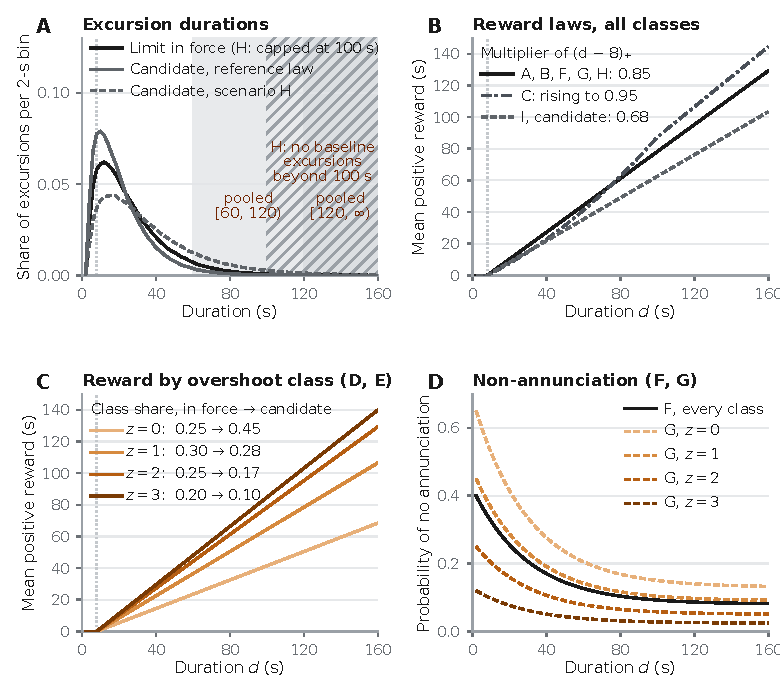
\includegraphics[width=\textwidth]{figures/FigureS6_simulation_laws.pdf}
\caption{The simulation's data-generating laws, drawn from the simulation code. A: share of excursions in each two-second duration bin at the limit in force and under the candidate limit for the reference law and for scenario H, in a draw of 20\,000 patients; the shaded bands are the pooled cells $[60,120)$ and $[120,\infty)$ of the simulation map, the dotted line the 8-second persistence clock, and the hatched region the durations beyond H's 100-second cap, where the candidate places excursions that no baseline cell contains. B: mean positive reward $m(d)$ for the laws without overshoot dependence. C: mean positive reward by overshoot class in D and E, with each class's share at the limit in force and under the candidate. D: probability that an excursion goes unannunciated in F (all classes) and G (by class).}
\label{sfig:simlaws}
\figalt{Four panels. The first shows right-skewed duration distributions peaking near 10 seconds, with the candidate distribution shorter than the baseline in the reference law and longer in scenario H, whose candidate extends past 100 seconds into a hatched region without baseline excursions. The second shows three straight reward lines rising from 8 seconds with slopes 0.85, up to 0.95 and 0.68. The third shows four lines of increasing slope for overshoot classes zero to three. The fourth shows non-annunciation probabilities decreasing with duration from 0.65 at short durations towards a floor near 0.05 to 0.15.}
\end{figure}
\begin{figure}[htbp]\centering
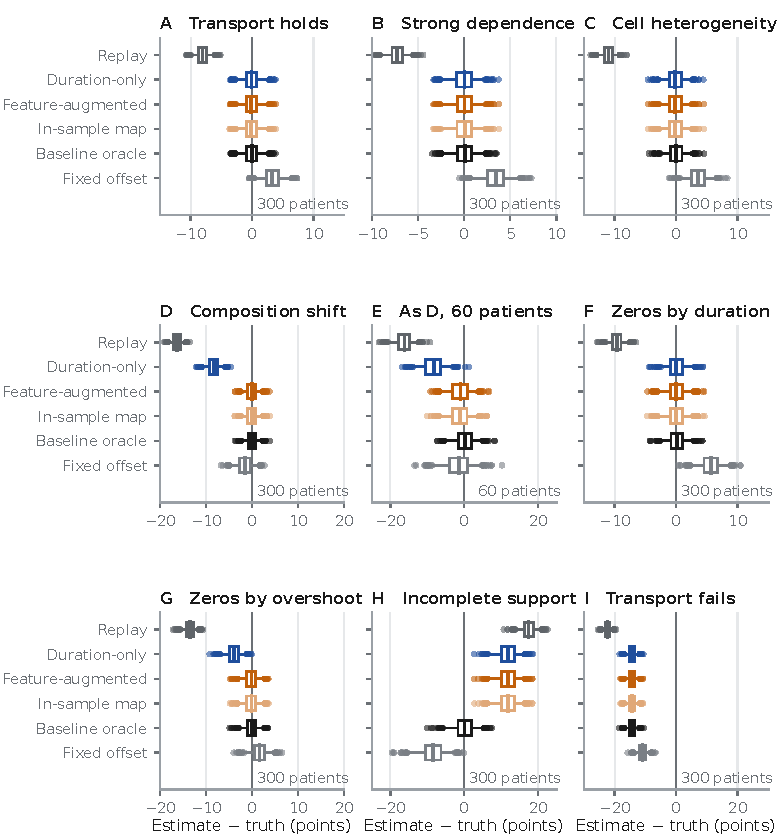
\includegraphics[width=\textwidth]{figures/FigureS7_simulation_replicates.pdf}
\caption{Replicate distributions of estimate minus truth for the six estimators in every scenario. The box spans the interquartile range, the line inside it is the median, the whiskers reach the 2.5th and 97.5th percentiles, and replicates beyond them are drawn individually; the horizontal scale differs between panels. Every panel uses 500 replicates.}
\label{sfig:simreps}
\figalt{Nine panels of horizontal box plots. Replay sits left of zero in every panel except H, where it sits to the right. The calibrated estimators and the oracle sit on zero in A, B, C, F and, for the feature-augmented estimator, in D, E and G; duration-only calibration sits left of zero in D, E and G. In H and I every calibrated estimator sits far from zero, with a box not much wider than in the other panels. The fixed-offset comparator is displaced in most panels.}
\end{figure}

% ---- end inline ----


% ---- inlined from 02_supp/../01_main/TAB_SIMULATION_SUPP.tex ----
\subsection{Data-generating laws}
Figure~\ref{sfig:simlaws} draws the laws that follow: the duration distributions at the two limits, the reward laws with and without overshoot dependence, and the non-annunciation probabilities of scenarios F and G.
Patient effects are $F_i=G_i/k$, where $G_i\sim\mathrm{Gamma}(k,1)$ independently, with $k=4$ except in scenario B, where $k=1.2$. Each patient has $N_i=\max\{1,\mathrm{Poisson}(25F_i)\}$ excursions. The same $N_i$ and $F_i$ are used at the baseline and candidate rules. Conditional on them, duration draws at the two rules are independent, with Gamma shape 1.6 and scale $s_uF_i^{0.3}$. The baseline scale is 14; the candidate scale is 11, except in H where it is 20. Durations are rounded upward to two-second values and capped at 400 seconds. In H only, baseline durations are capped at 100 seconds, producing a point mass there and leaving some candidate cells unobserved at baseline. These experiments simulate excursion measures, not a nested pair of sample paths.
Overshoot classes $z=0,1,2,3$ have baseline probabilities $(0.25,0.30,0.25,0.20)$. Candidate probabilities are unchanged in A, B, C and H and equal $(0.45,0.28,0.17,0.10)$ otherwise. Define $b(d)=(d-8)_+$ and a mean positive reward $m(d,z)=b(d)g(d,z)$. The multiplier is 0.85 in A, B, F, G, H and I; it is $(0.45,0.70,0.85,0.92)_z$ in D and E and $\min\{0.95,0.55+0.004d\}$ in C. In I, the candidate reward is additionally multiplied by 0.8. Baseline positive rewards are Gamma with scale 3 and shape $m/3$, up to a numerical shape guard of order $10^{-9}$; rewards with $m=0$ are set to zero.
Scenarios F and G add stochastic non-annunciation: the positive reward is replaced by zero with probability $p(d,z)$. In F, $p=0.40\{0.20+0.80\exp[-(d-2)/30]\}$; in G, 0.40 is replaced by $(0.65,0.45,0.25,0.12)_z$. Thus the conditional mean is $a_u(d,z)=\{1-p(d,z)\}m_u(d,z)$. The same cells can contain both observed zeros and positive rewards. No positivity assumption on $a_0$ is imposed.
The simulation map has 30 nominal two-second bins below 60 seconds and pooled bins $[60,120)$ and $[120,\infty)$. It uses the same count/seconds carrier functions as the clinical analysis but a smaller partition. Feature-map selection uses a minimum of five excursions. Scenario E uses 60 patients to examine sparse cells; all other main scenarios use 300. Independent map selection uses an additional sample of the same size. A secondary analysis selects the map within the estimation sample. The baseline-reward oracle integrates the known $a_0(d,z)$ excursion by excursion, including where baseline observations are absent. In I this oracle still uses the baseline reward, so it does not know the deliberately changed candidate reward. The fixed-offset comparator matches observed baseline linked seconds with a persistence model, using mean duration within each pooled cell.
\subsection{Complete estimator comparisons}
Table~\ref{stab:simfull} gives bias, empirical standard deviation, root mean squared error, coverage and the Monte Carlo standard error of the bias for all six estimators in every scenario; Figure~\ref{sfig:simreps} shows the replicate distributions behind it. Three features are visible there that the summary statistics compress. Wherever the calibrated estimators are unbiased (A, B, C, F), their empirical standard deviation is within 0.05 points of the baseline-reward oracle's, so nothing is lost by estimating the reward instead of knowing it. The map selected in sample reproduces the independently selected map almost replicate by replicate: the two biases differ by at most 0.13 points in any scenario. In H and I the whole distribution of every estimator moves away from zero by several times its width: the feature-augmented bias is 11.76 points in H and -14.36 in I against empirical standard deviations of 2.56 and 1.33, which is why the intervals in those scenarios are narrow and wrong at once.
\begin{longtable}{@{}llrrrrr@{}}
\caption{Simulation accuracy and Monte Carlo uncertainty.}\label{stab:simfull}\\
\toprule Method & & Bias & Empirical SD & RMSE & Coverage & MCSE(bias)\\\midrule\endfirsthead
\toprule Method & & Bias & Empirical SD & RMSE & Coverage & MCSE(bias)\\\midrule\endhead
\bottomrule\endfoot
\multicolumn{7}{@{}l}{\textbf{A: Transport holds}; truth 28.571\%, $n=300$}\\
Replay & & -8.07 & 0.99 & 8.13 & --- & 0.046\\
Duration-only & & -0.09 & 1.34 & 1.34 & 0.935 & 0.061\\
Feature-augmented & & -0.08 & 1.34 & 1.34 & 0.935 & 0.061\\
Feature map selected in sample & & -0.08 & 1.34 & 1.34 & 0.932 & 0.061\\
Baseline-reward oracle & & -0.05 & 1.33 & 1.33 & --- & 0.061\\
Fixed-offset comparator & & 3.31 & 1.49 & 3.63 & --- & 0.068\\
\addlinespace
\multicolumn{7}{@{}l}{\textbf{B: Stronger patient dependence}; truth 27.885\%, $n=300$}\\
Replay & & -7.26 & 0.92 & 7.32 & --- & 0.043\\
Duration-only & & -0.02 & 1.20 & 1.20 & 0.940 & 0.055\\
Feature-augmented & & -0.02 & 1.20 & 1.20 & 0.938 & 0.055\\
Feature map selected in sample & & -0.02 & 1.20 & 1.20 & 0.938 & 0.055\\
Baseline-reward oracle & & 0.02 & 1.20 & 1.20 & --- & 0.055\\
Fixed-offset comparator & & 3.39 & 1.35 & 3.65 & --- & 0.061\\
\addlinespace
\multicolumn{7}{@{}l}{\textbf{C: Pooled-cell heterogeneity}; truth 31.562\%, $n=300$}\\
Replay & & -11.01 & 0.97 & 11.05 & --- & 0.045\\
Duration-only & & -0.14 & 1.42 & 1.43 & 0.935 & 0.065\\
Feature-augmented & & -0.14 & 1.43 & 1.43 & 0.930 & 0.065\\
Feature map selected in sample & & -0.14 & 1.43 & 1.43 & 0.927 & 0.065\\
Baseline-reward oracle & & 0.02 & 1.41 & 1.41 & --- & 0.064\\
Fixed-offset comparator & & 3.54 & 1.58 & 3.87 & --- & 0.072\\
\addlinespace
\multicolumn{7}{@{}l}{\textbf{D: Overshoot and composition shift}; truth 36.904\%, $n=300$}\\
Replay & & -16.35 & 0.98 & 16.38 & --- & 0.045\\
Duration-only & & -8.37 & 1.33 & 8.47 & 0.000 & 0.060\\
Feature-augmented & & -0.06 & 1.25 & 1.25 & 0.945 & 0.057\\
Feature map selected in sample & & -0.05 & 1.25 & 1.25 & 0.943 & 0.057\\
Baseline-reward oracle & & 0.01 & 1.22 & 1.22 & --- & 0.056\\
Fixed-offset comparator & & -1.59 & 1.63 & 2.28 & --- & 0.074\\
\addlinespace
\multicolumn{7}{@{}l}{\textbf{E: Sparse feature cells}; truth 36.908\%, $n=60$}\\
Replay & & -16.34 & 2.14 & 16.48 & --- & 0.096\\
Duration-only & & -8.29 & 2.85 & 8.77 & 0.142 & 0.128\\
Feature-augmented & & -1.08 & 2.74 & 2.94 & 0.943 & 0.123\\
Feature map selected in sample & & -1.22 & 2.78 & 3.04 & 0.940 & 0.125\\
Baseline-reward oracle & & 0.15 & 2.68 & 2.68 & --- & 0.120\\
Fixed-offset comparator & & -1.57 & 3.53 & 3.86 & --- & 0.158\\
\addlinespace
\multicolumn{7}{@{}l}{\textbf{F: Duration-dependent zero inflation}; truth 30.283\%, $n=300$}\\
Replay & & -9.65 & 1.02 & 9.70 & --- & 0.047\\
Duration-only & & 0.07 & 1.44 & 1.44 & 0.940 & 0.065\\
Feature-augmented & & 0.04 & 1.46 & 1.46 & 0.935 & 0.067\\
Feature map selected in sample & & 0.04 & 1.47 & 1.46 & 0.932 & 0.067\\
Baseline-reward oracle & & 0.13 & 1.41 & 1.42 & --- & 0.064\\
Fixed-offset comparator & & 5.67 & 1.67 & 5.91 & --- & 0.076\\
\addlinespace
\multicolumn{7}{@{}l}{\textbf{G: Feature-dependent zero inflation}; truth 34.006\%, $n=300$}\\
Replay & & -13.50 & 1.04 & 13.54 & --- & 0.048\\
Duration-only & & -3.92 & 1.45 & 4.18 & 0.195 & 0.066\\
Feature-augmented & & -0.15 & 1.42 & 1.43 & 0.915 & 0.065\\
Feature map selected in sample & & -0.16 & 1.42 & 1.43 & 0.912 & 0.065\\
Baseline-reward oracle & & -0.06 & 1.40 & 1.40 & --- & 0.064\\
Fixed-offset comparator & & 1.60 & 1.69 & 2.33 & --- & 0.077\\
\addlinespace
\multicolumn{7}{@{}l}{\textbf{H: Incomplete support}; truth -59.151\%, $n=300$}\\
Replay & & 17.53 & 1.82 & 17.62 & --- & 0.085\\
Duration-only & & 11.75 & 2.56 & 12.03 & 0.010 & 0.117\\
Feature-augmented & & 11.76 & 2.56 & 12.03 & 0.010 & 0.117\\
Feature map selected in sample & & 11.76 & 2.55 & 12.03 & 0.010 & 0.117\\
Baseline-reward oracle & & 0.05 & 2.75 & 2.75 & --- & 0.125\\
Fixed-offset comparator & & -8.56 & 3.20 & 9.13 & --- & 0.145\\
\addlinespace
\multicolumn{7}{@{}l}{\textbf{I: Reward transport fails}; truth 42.862\%, $n=300$}\\
Replay & & -22.35 & 0.98 & 22.37 & --- & 0.045\\
Duration-only & & -14.37 & 1.30 & 14.43 & 0.000 & 0.059\\
Feature-augmented & & -14.36 & 1.33 & 14.42 & 0.000 & 0.060\\
Feature map selected in sample & & -14.36 & 1.33 & 14.42 & 0.000 & 0.060\\
Baseline-reward oracle & & -14.33 & 1.29 & 14.39 & --- & 0.058\\
Fixed-offset comparator & & -10.97 & 1.47 & 11.07 & --- & 0.066\\
\addlinespace
\end{longtable}
Bias, empirical standard deviation and root mean squared error are percentage points. Bias MCSE combines the independent replicate mean and population-truth Monte Carlo errors. Coverage has binomial MCSE $\{\widehat c(1-\widehat c)/400\}^{1/2}$ conditional on the estimated truth. The common truth error is assessed separately by rescoring the saved intervals one truth MCSE above and below its estimate; that sensitivity range is not an additional formally estimated coverage standard error.
\subsection{Truth precision, overlap and observed zeros}
Table~\ref{stab:simdiag} records the precision of the population truths and three sample diagnostics. The truth Monte Carlo standard error is between 0.0091 and 0.0230 points, small against every bias the tables report. Observed zeros make up 18.4--19.8\% of excursions where they arise from the persistence clock alone and 37.3--38.1\% under stochastic non-annunciation (F, G). The share of candidate replayed time in duration bins with no baseline excursion is zero in every scenario except H (5.9\%), where it is the identification failure by construction. Between 3.6\% and 6.3\% of the cells of the independently selected map are coarsened to their parent duration rate in the 300-patient scenarios, against 24.8\% in E, where 60 patients leave many cells below the five-excursion minimum.
\begin{table}[htbp]\centering\small
\caption{Population-truth precision and sample diagnostics.}\label{stab:simdiag}
\begin{tabular}{@{}lrrrr@{}}\toprule
Scenario & Truth MCSE & Zero rewards (\%) & Unobserved duration share (\%) & Coarsened cells (\%)\\\midrule
A & 0.0113 & 19.7 & 0.0 & 5.4\\
B & 0.0113 & 18.4 & 0.0 & 3.6\\
C & 0.0124 & 19.7 & 0.0 & 5.4\\
D & 0.0107 & 19.7 & 0.0 & 5.5\\
E & 0.0107 & 19.8 & 0.0 & 24.8\\
F & 0.0119 & 38.1 & 0.0 & 5.4\\
G & 0.0115 & 37.3 & 0.0 & 5.4\\
H & 0.0230 & 19.7 & 5.9 & 6.3\\
I & 0.0091 & 19.7 & 0.0 & 5.5\\
\bottomrule\end{tabular}
\tightnote{Truth MCSE is in percentage points, based on four million independent patients for each scenario. Unobserved duration share is target replayed time in bins without baseline observations. Coarsened cells is a proportion of cells in the independently selected feature map, not a proportion of burden. Zero-reward shares are averages over the simulated estimation samples.}
\end{table}
\subsection{Patient-count sensitivity}
Table~\ref{stab:simsweep} and panels C and D of Figure 2 in the main manuscript follow the feature-augmented estimator as the patient count grows. In A the empirical standard deviation falls from 1.327 points at 300 patients to 0.420 at 2\,400 (0.469 expected at the $n^{-1/2}$ rate), coverage moves from 0.935 to 0.970, and the ratio of the mean bootstrap standard error to the empirical standard deviation stays between 0.98 and 1.11. In G, with feature-dependent non-annunciation, coverage is 0.943 and 0.925 at 600 and 1\,200 patients, with mean bootstrap standard error to empirical standard deviation ratios of 1.03 and 0.94. The bootstrap therefore tracks the sampling variability at every count examined, and the coverage shortfall at 300 patients is not accompanied by a bias that grows with the sample.
\begin{table}[htbp]\centering\small
\caption{Independent-map feature calibration as patient count increases.}\label{stab:simsweep}
\begin{tabular}{@{}llrrrrr@{}}\toprule
Scenario & Patients & Bias & Empirical SD & Coverage & MCSE(coverage) & Mean SE/SD\\\midrule
A & 300 & -0.090 & 1.327 & 0.935 & 0.012 & 0.992\\
A & 600 & -0.103 & 0.951 & 0.930 & 0.013 & 0.980\\
A & 1200 & -0.041 & 0.673 & 0.940 & 0.012 & 0.982\\
A & 2400 & -0.015 & 0.420 & 0.970 & 0.009 & 1.107\\
G & 600 & -0.209 & 0.958 & 0.943 & 0.012 & 1.026\\
G & 1200 & -0.113 & 0.731 & 0.925 & 0.013 & 0.944\\
\bottomrule\end{tabular}
\tightnote{Each row uses 400 replicates, with 200 patient bootstrap resamples per replicate. Mean SE/SD compares the mean bootstrap standard error with empirical variability. A uses a common duration-only reward; G includes feature-dependent stochastic non-annunciation. Rows use the same scenario-specific high-precision population truth.}
\end{table}

% ---- end inline ----


\section{Descriptive fixed-offset comparisons}\label{s:level}

% ---- inlined from 02_supp/_blocks/S16_level_fixedoffset.tex ----
At the four-second calibration convention, replayed-to-recorded burden ratios on the fitting subsample are 2.46 (95\% interval 2.22--2.79), 1.67 (1.59--1.74), 2.07 (1.80--2.43) and 1.51 (1.23--1.89). Under the 30-second recorded-run convention on the same admissions, the point estimates are 2.73, 1.75, 2.32 and 1.48. These estimates use different admissions from the held-out ratios in the main paper and need not coincide.

Linked and unlinked recorded seconds provide exact accounting under a fixed convention, not prediction of unobserved device behaviour. The baseline unlinked shares are approximately 9\%, 13\%, 14\% and 25\%. The candidate unlinked share is not identified by replay.

Fixed-offset calculations are retained only as descriptive sensitivity analyses. At a one-step less stringent limit, the reductions obtained from the offset values in Table~\ref{tab:level} span 44.4--44.7\%, 28.9--29.9\%, 36.7--44.0\% and 83.2--84.2\%. This span is neither an identified set nor a confidence interval. Agreement with some cell-calibrated estimates does not establish that a monitor implements a persistence rule; marginal onset lag, long-duration linkage probability and total linked seconds describe different features of its recorded output.

% ---- inlined from 02_supp/../01_main/TABLE_LEVEL_SUPP.tex ----
\begin{table}[htbp]\centering\scriptsize
\setlength{\tabcolsep}{2.6pt}
\caption{The level, on the admissions the pairs come from. $\hat\rho_4$ is replayed excursion seconds over
recorded annunciation seconds with both sides merged at 4\,s (the theory's convention), $\hat\rho_{30}$ the
same admissions under the 30-s convention, and `test' the held-out result, analysed once under the design fixed in advance, of
Figure 3 of the main manuscript of the main text (30-s convention, different admissions). `Unlinked' is the share of recorded
annunciation seconds attached to no excursion, and $\hat\rho_4^{\mathrm{linked}}$ the ratio with only
linked seconds in the denominator, which is $\mathbb E[D]/\mathbb E[\hat\psi_{\mathrm m}(D)]$ exactly.
Three fixed offsets summarize the device as a persistence rule: the median onset lag among linked
excursions (`raw', read under the 30-second convention of this column block; under the 4-second
convention it is $18$, $4$, $2$ and $2$\,s), the offset $\theta_{\mathrm m}$ that reproduces the linked annunciation seconds, and
the offset $\theta^\ast$ that reproduces $\hat\rho_4$ given $\hat q$. The last columns are the replayed
reduction at one less stringent step and the range of corrected reductions over the three offsets: the
fixed-offset calibration range of Section~\ref{s:level} (the monotone map of Lemma~A12 of the \emph{Technical Appendix}, Section~A.4.3
evaluated at the offsets a persistence reading of the device would use; not an identified set).}
\label{tab:level}
\begin{tabular}{@{}lllllrrrrrr@{}}
\toprule
 & \multicolumn{3}{c}{Level $\rho$ (95\% CI)} & & & \multicolumn{3}{c}{Fixed offset (s)} & \multicolumn{2}{c}{Reduction, $+1$} \\
\cmidrule(lr){2-4}\cmidrule(lr){7-9}\cmidrule(lr){10-11}
Channel & $\hat\rho_4$ & $\hat\rho_{30}$ & test & Unl. & $\hat\rho_4^{\mathrm{lk}}$ & raw & $\theta_{\mathrm m}$ & $\theta^\ast$ & replayed & range \\
\midrule
RR low & 2.46 (2.22--2.79) & 2.73 (2.44--3.14) & 2.53 (2.27--2.82) & 9\% & 2.71 & 18 & 17.8 & 14.9 & 41.2\% & 44.4--44.7\% \\
\SpO{} low & 1.67 (1.59--1.74) & 1.75 (1.66--1.83) & 1.65 (1.57--1.74) & 13\% & 1.91 & 12 & 14.7 & 5.8 & 28.1\% & 28.9--29.9\% \\
HR high & 2.07 (1.80--2.43) & 2.32 (1.99--2.73) & 2.23 (1.94--2.58) & 14\% & 2.40 & 2 & 13.5 & 7.4 & 35.0\% & 36.7--44.0\% \\
HR low & 1.51 (1.23--1.89) & 1.48 (1.20--1.86) & 1.72 (1.32--2.41) & 25\% & 2.02 & 2 & 23.4 & none & 82.0\% & 83.2--84.2\% \\
\bottomrule
\end{tabular}
\tightnote{Intervals are patient-cluster bootstraps ($B=400$). The three
offsets differ because the device behaves most nearly as a persistence device on respiration rate low,
where the annunciation ratio is near zero below $18$\,s and then rises sharply; on the other channels it
rises gradually and long excursions are annunciated only in part, which a single delay
constant fitted to the median lag cannot carry (Section~\ref{s:level}).}
\end{table}

% ---- end inline ----


% ---- end inline ----




\section{Technical identification result}\label{s:technical}
This result is included as technical support for the calibration framework rather than as a primary contribution of the paper. Let $\nu_u(A)$ denote the mean number of excursions per unit monitored exposure whose $(D,Z)$ values fall in $A$, and let $\mu_u(A)$ denote the corresponding mean linked alarm seconds. When $\mu_u\ll\nu_u$, write $a_u=d\mu_u/d\nu_u$. The linked burden is $B_{\mathrm m}(u)=\int a_u\,d\nu_u$.

\newtheorem{theorem}{Theorem}
\begin{theorem}[Zero-inclusive identification and standardisation]\label{thm:supp-ident}
Suppose the observed numerical stream enumerates every eligible baseline excursion, the recorded alarm log covers the same period, and a fixed measurable linkage rule assigns each alarm run to at most one excursion. Let $Y$ be an excursion's total linked alarm seconds, with $Y=0$ when no run is assigned, and assume the relevant mean measures are finite.
\begin{enumerate}\itemsep2pt
\item[(i)] The baseline reward $a_0(d,z)=\mathbb E(Y\mid D=d,Z=z)$ is identified $\nu_{u_0}$-almost everywhere; its duration-marginal counterpart $\bar a_0(d)$ is likewise identified.
\item[(ii)] Under joint reward transport and overlap $\nu_{u_1}\ll\nu_{u_0}$, the candidate linked burden is $B_{\mathrm m}(u_1)=\int a_0\,d\nu_{u_1}$. Under duration transport and duration overlap, the corresponding candidate burden is $\int \bar a_0\,d\nu^D_{u_1}$.
\item[(iii)] Let $U(u)$ be recorded alarm seconds per unit exposure that remain unassigned to any eligible excursion and let $q_u=U(u)/\{B_{\mathrm m}(u)+U(u)\}$. Then
\[
\Delta_{\mathrm{recorded}}=\Delta_{\mathrm m}\frac{1-q_{u_0}}{1-q_{u_1}}.
\]
Thus linked and total-recorded relative burden coincide only when the unlinked share is stable across rules, or under another explicit assumption that identifies the candidate unlinked share.
\end{enumerate}
\end{theorem}

\begin{proof}
Because the complete baseline excursion list is observed and non-linked excursions are assigned the observed value $Y=0$, the joint excursion-level law of $(D,Z,Y)$ is observed under the baseline linkage convention. Hence its conditional mean $\mathbb E(Y\mid D,Z)$ is identified almost everywhere. Parts (ii) follow by standardisation of this identified reward over the replayed candidate excursion measure under the stated transport and absolute-continuity conditions. For part (iii), total recorded burden equals $B_{\mathrm m}(u)+U(u)=B_{\mathrm m}(u)/(1-q_u)$; taking the candidate-to-baseline ratio gives the displayed identity.
\end{proof}

The theorem makes explicit what is observed and what remains assumption-dependent. It does not identify the alarm process under an unimplemented rule without transport, does not validate the linkage convention, and does not convert the sensitivity specifications into bounds.

\bibliographystyle{unsrtnat}\bibliography{refs}
\end{document}
